\documentclass{beamer}
\usepackage{ctex, hyperref}
\usepackage[T1]{fontenc}
\usepackage[french]{babel}
\usepackage{amssymb}

% other packages
\usepackage{latexsym,amsmath,xcolor,multicol,booktabs,calligra}
\usepackage{graphicx,pstricks,listings,stackengine}
\usepackage[font=tiny]{caption}

\author{Eoin Brereton Hurley}
\title{MIND 1024}
\subtitle{Histoire de l'Informatique}
\institute{Université Grenoble Alpes}
\date{30/06/2022}
\usepackage{NJUPT}

% defs
\def\cmd#1{\texttt{\color{red}\footnotesize $\backslash$#1}}
\def\env#1{\texttt{\color{blue}\footnotesize #1}}
\definecolor{deepblue}{rgb}{0,0,0.5}
\definecolor{deepred}{rgb}{0.6,0,0}
\definecolor{deepgreen}{rgb}{0,0.5,0}
\definecolor{halfgray}{gray}{0.55}
\definecolor{darkpurple}{rgb}{0.5,0,0.6}

\lstset{
    basicstyle=\ttfamily\small,
    keywordstyle=\bfseries\color{deepblue},
    emphstyle=\ttfamily\color{deepred},    % Custom highlighting style
    stringstyle=\color{deepgreen},
    numbers=left,
    numberstyle=\small\color{halfgray},
    rulesepcolor=\color{red!20!green!20!blue!20},
    frame=shadowbox,
}


\begin{document}

\kaishu
\begin{frame}
    \titlepage
    \begin{figure}[htpb]
        \begin{center}
            
\includegraphics[width=0.75\linewidth]{pic/Logos-UGA.jpeg}
        \end{center}
    \end{figure}
\end{frame}

\begin{frame}
    \tableofcontents[sectionstyle=show,subsectionstyle=show/shaded/hide,subsubsectionstyle=show/shaded/hide]
\end{frame}


\section{Introduction}

\subsection{Aperçu de la Machine}

\begin{frame}{Machine Neuronale MIND 1024}
    \begin{columns}[T]
        \column{0.65\textwidth}
            \scriptsize
            \begin{itemize}[<+-| alert@+>] % 当然,除了alert,手动在里面插 \pause 也行
                \item MIND signifie \textit{Machine à Interaction Neuronale Démodulée}
                \item Cette machine simule un réseau de \textit{Hopfield}, (il s'agit d'un type spécifique du réseau de neurones récurrents)
                \item Le réseau consiste en 1024 neurones interconnectés mis en \oe uvre à l'aide de 1 048 576 synapses.
                \item Précisions sur le réseau \textit{Hopfield} plus tard...
                \item Maintenant : du contexte historique !
            \end{itemize}
            \begin{columns}[T]
                \column{0.50\textwidth}
                    \begin{figure}
                    \centering
                    \includegraphics[width=0.65\linewidth]{pic/Exemple de Carte Mère.jpeg}
                    \caption{Détail 1 du MIND 1024}
                    \end{figure}
                \column{0.45\textwidth}
                    \begin{figure}
                    \centering
                    \includegraphics[width=0.75\linewidth]{pic/Détail 1.jpeg}
                    \caption{Exemple de Carte Mère du MIND 1024}
                    \end{figure}
            \end{columns}
        \column{0.35\textwidth}
            \begin{figure}
            \centering
                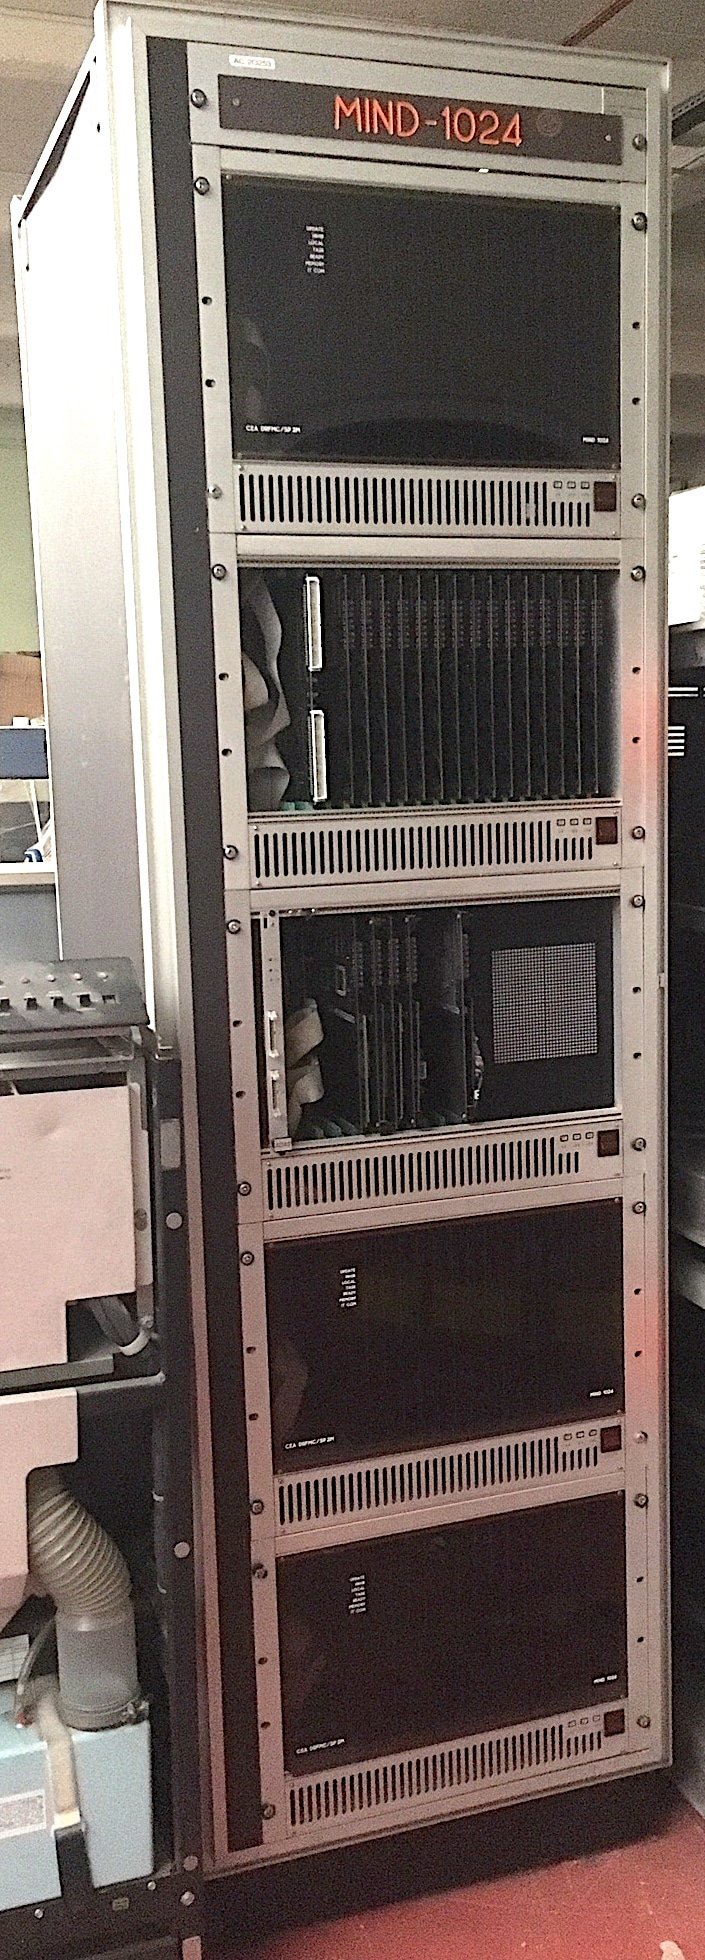
\includegraphics[width=0.5\linewidth]{pic/Vue d'Ensemble.jpeg}
                \caption{Vue d'Ensemble du MIND 1024}
            \end{figure}
    \end{columns}
\end{frame}

\subsection{Contexte Historique}

\begin{frame}{Machine Neuronale MIND 1024}
    \begin{itemize}[<+-| alert@+>] % 当然,除了alert,手动在里面插 \pause 也行
        \item Problèmes avec les ordinateurs au 20e siècle :
            \begin{itemize}[<+-| alert@+>] % 当然,除了alert,手动在里面插 \pause 也行
                \item Bien qu'ils fassent très bien les calculs, à l'époque ils avaient de nombreux défauts.
            \end{itemize}
        \item Par exemple, tâches triviales pour les humains, mais difficiles pour les ordinateurs :
            \begin{itemize}[<+-| alert@+>] % 当然,除了alert,手动在里面插 \pause 也行
                \item Reconnaissance du visage,
                \item Identification des images,
                \item Compréhension de la voix, etc.
            \end{itemize}
            \begin{columns}[T]
                \column{0.35\textwidth}
                \begin{figure}
                \centering
                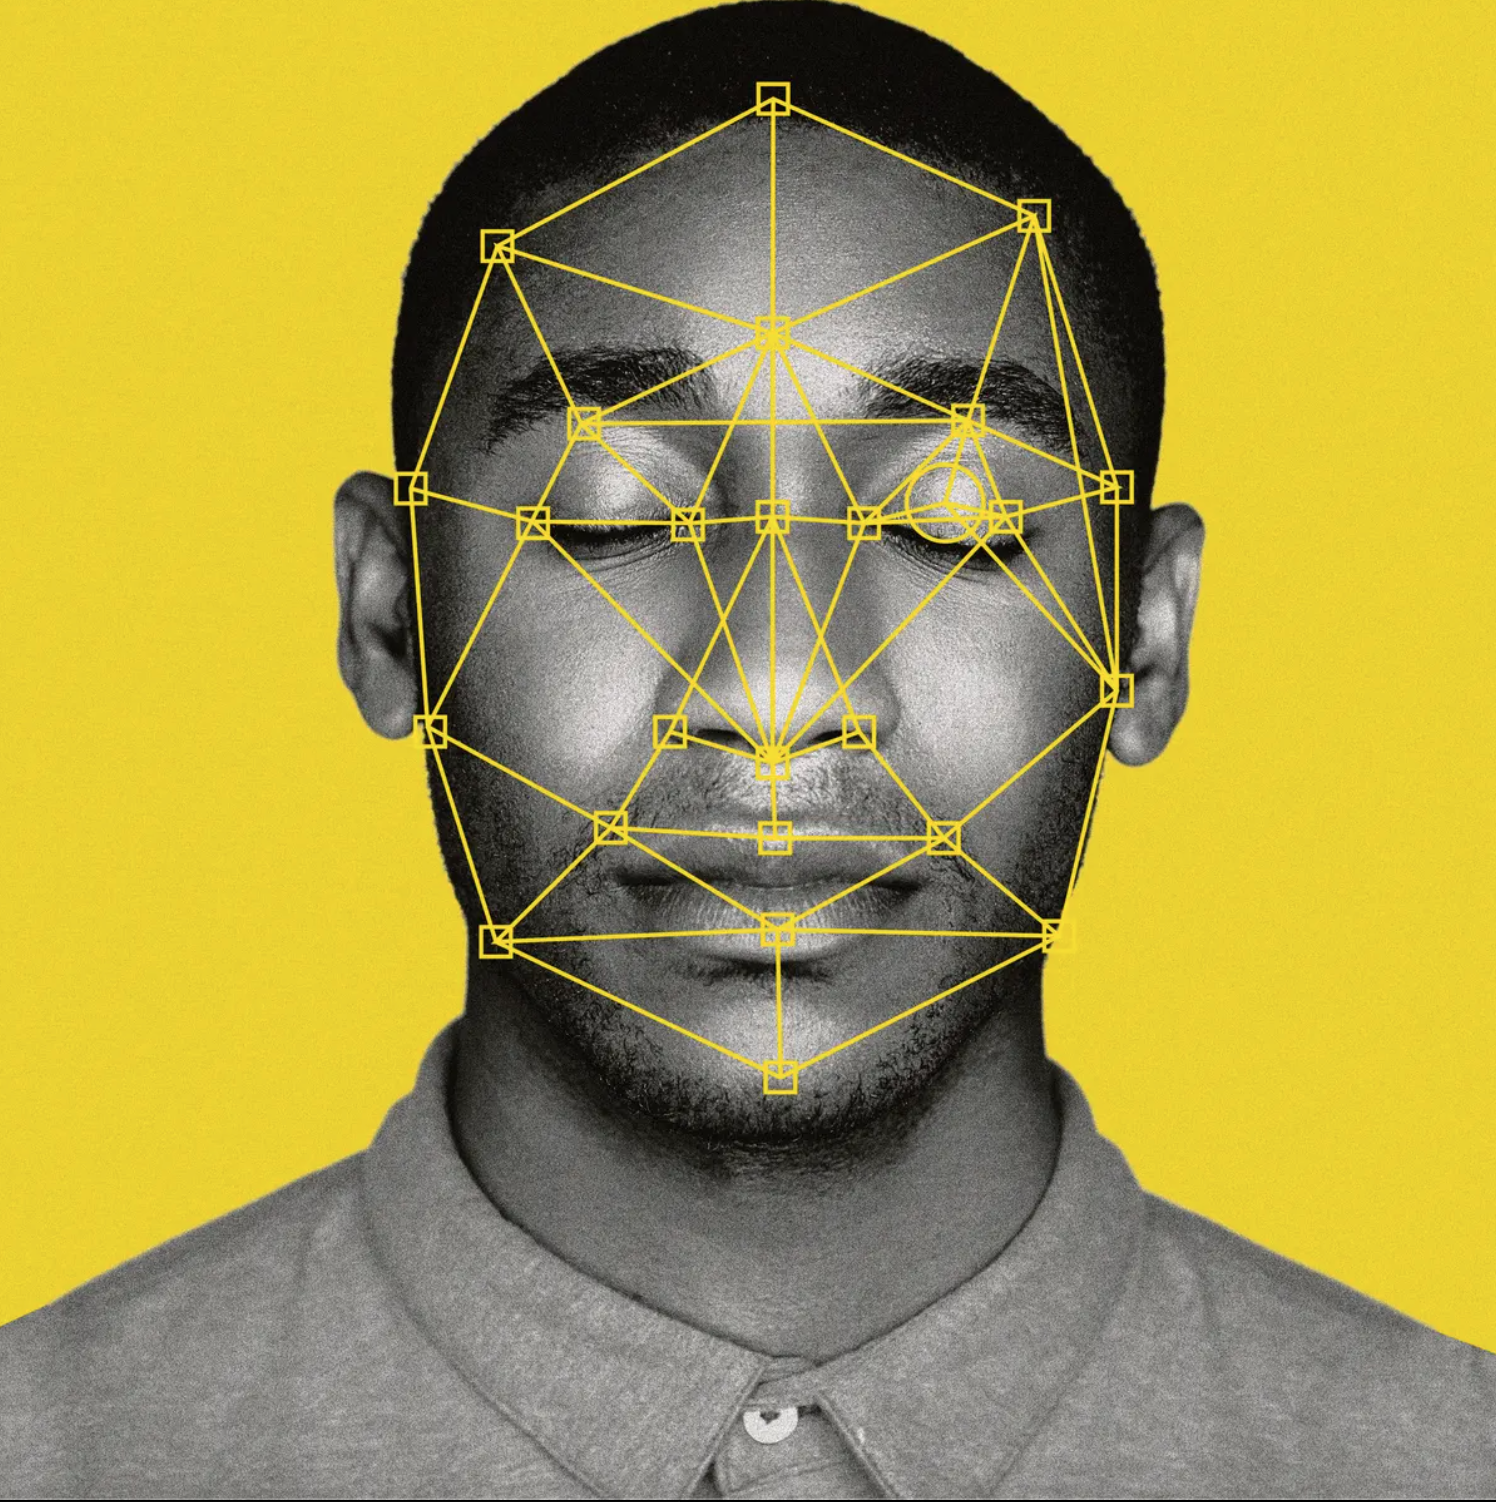
\includegraphics[width=0.65\linewidth]{pic/Reconnaissance-du-visage.png}
                \end{figure}
                \column{0.25\textwidth}
                \begin{figure}
                \centering
                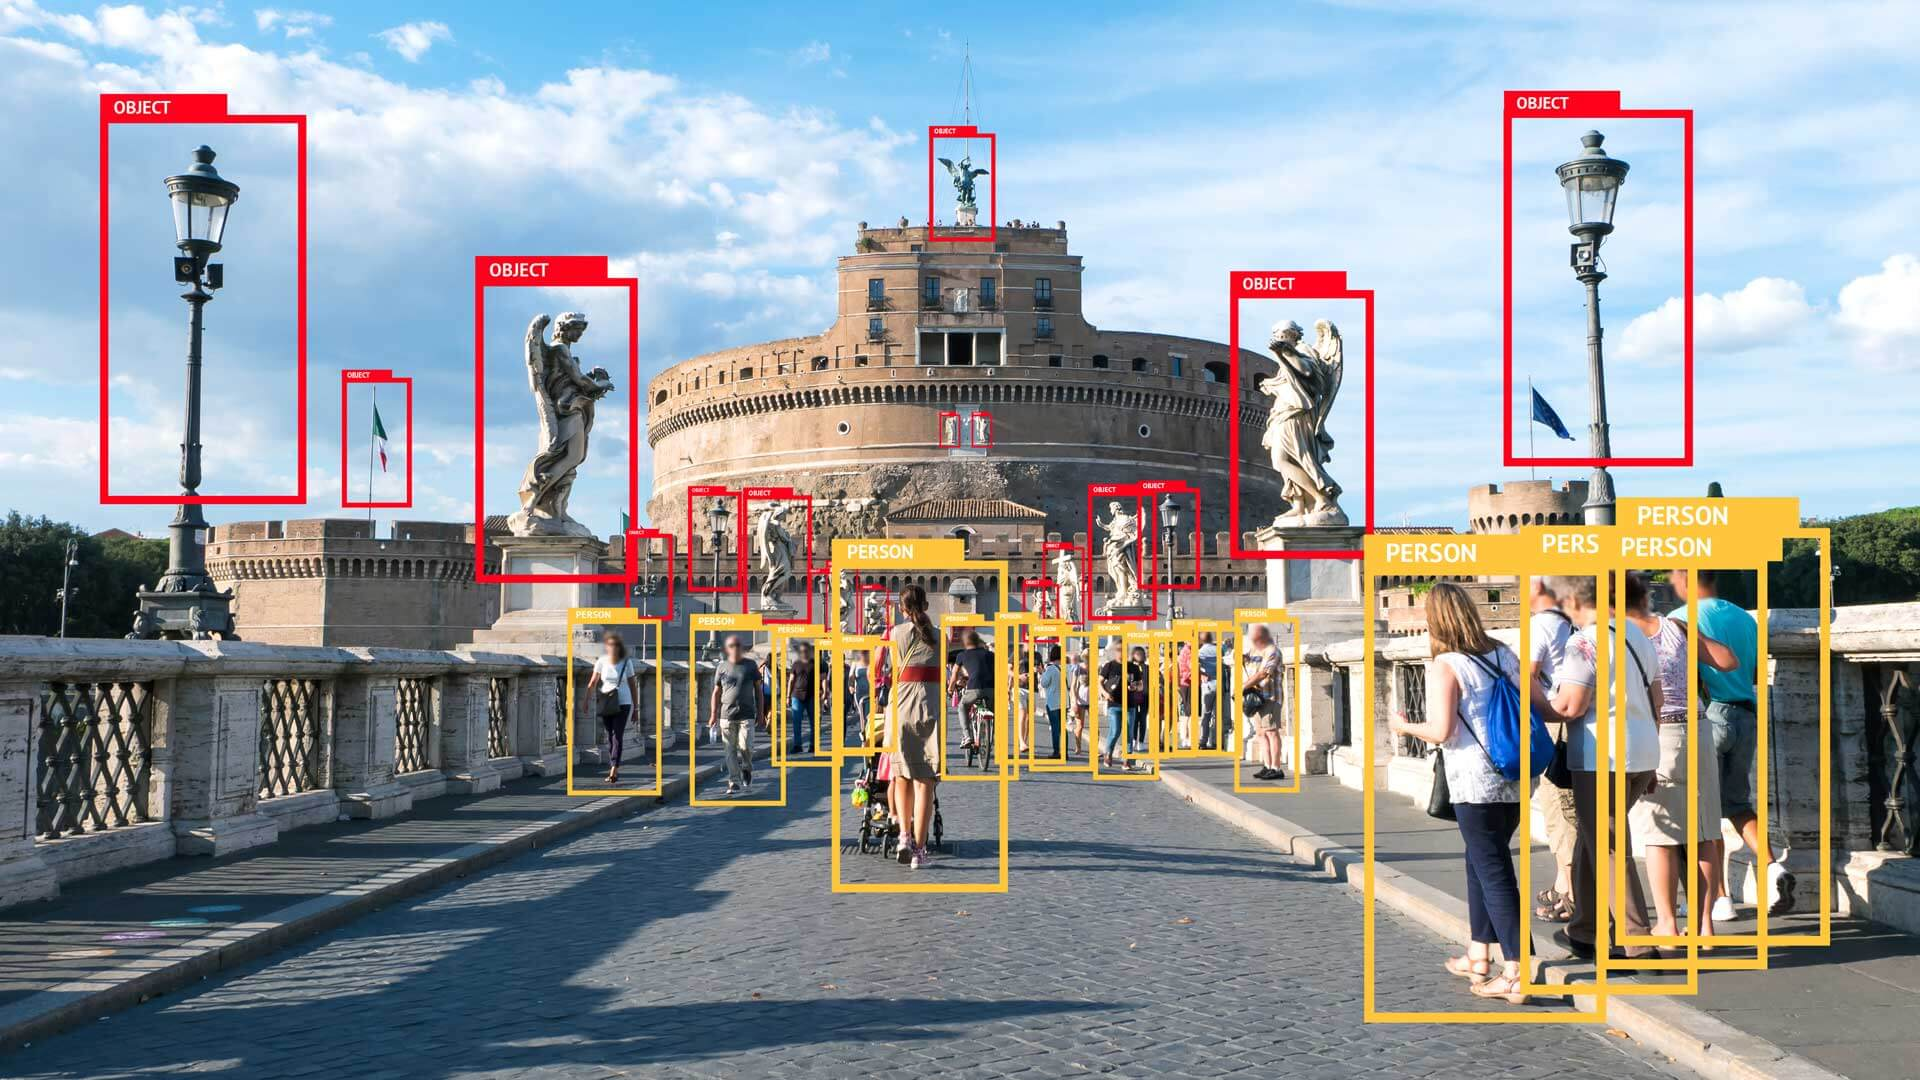
\includegraphics[width=1.2\linewidth]{pic/Identification-des-images.jpeg}
                \end{figure}
                \column{0.45\textwidth}
                \begin{figure}
                \centering
                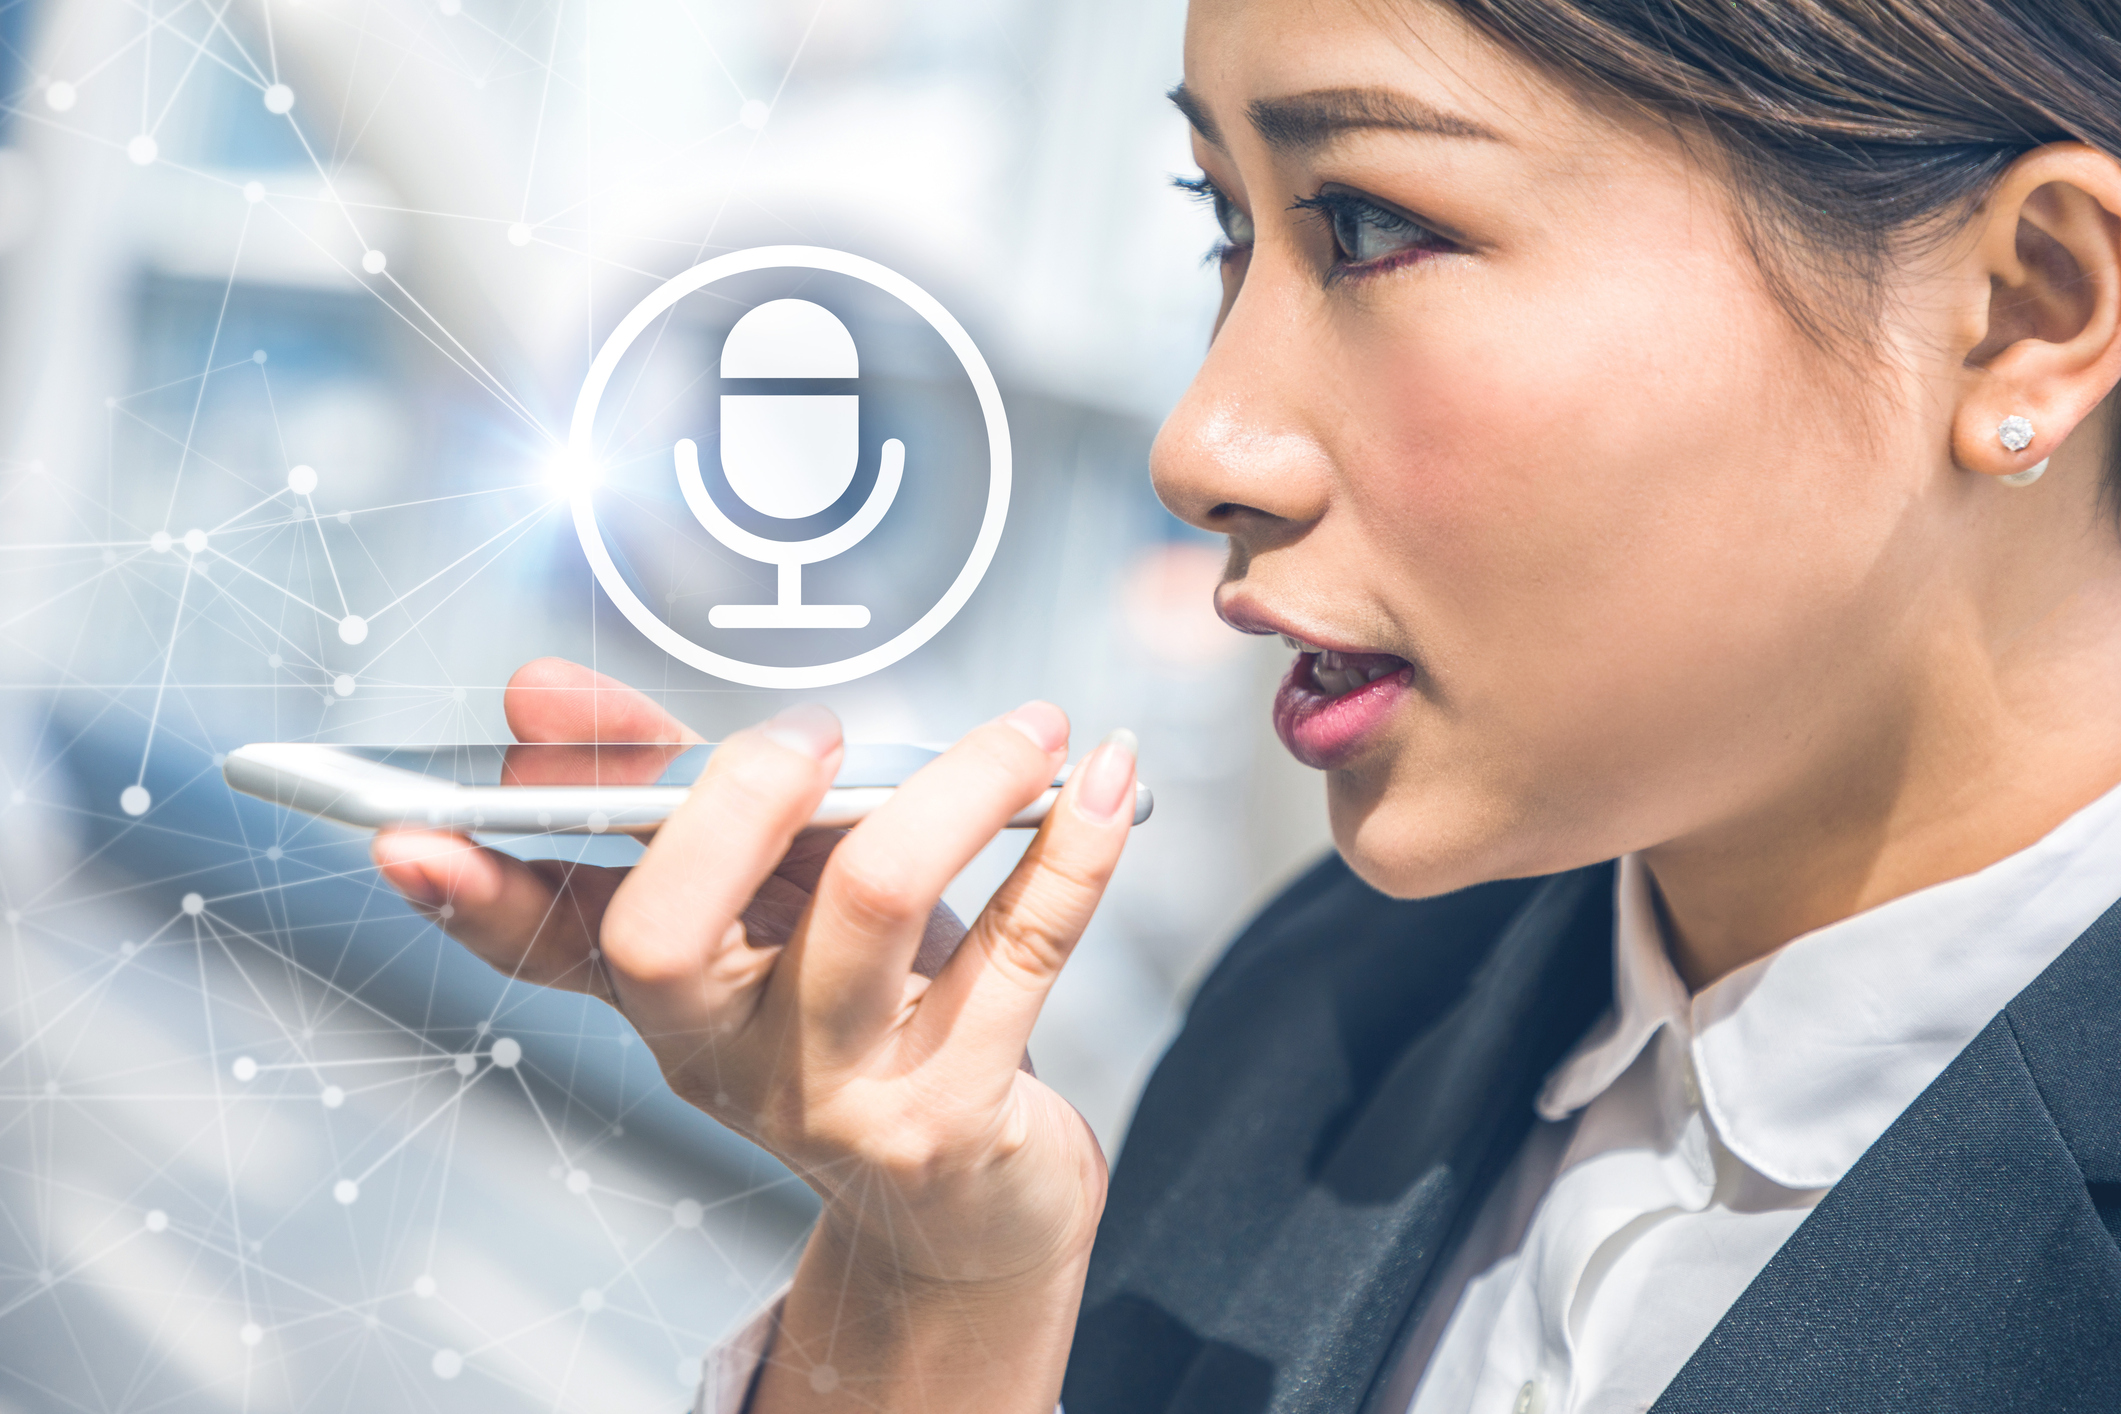
\includegraphics[width=0.65\linewidth]{pic/Reconnaissance-de-la-voix.jpeg}
                \end{figure}
            \end{columns}
    \end{itemize}
\end{frame}

\subsubsection{Alan Turing}

\begin{frame}{Machine Neuronale MIND 1024}
    \begin{columns}[T]
        \column{0.5\textwidth}
            \begin{itemize}[<+-| alert@+>] % 当然,除了alert,手动在里面插 \pause 也行
                \item En 1950, (35 ans avant la construction du MIND 1024)...
                \item \textit{Alan Turing} publie un article fondateur sur l'intelligence des machines à calcul.
                \item Il s'agit de l'artice dans lequel il a introduit le \textit{test de Turing, (initialement, le jeu d'imitation)}.
                \item C'est un test très bien connu qui permet de déterminer si une machine peut penser.
            \end{itemize}
        \column{0.5\textwidth}
            \begin{figure}
                \centering
                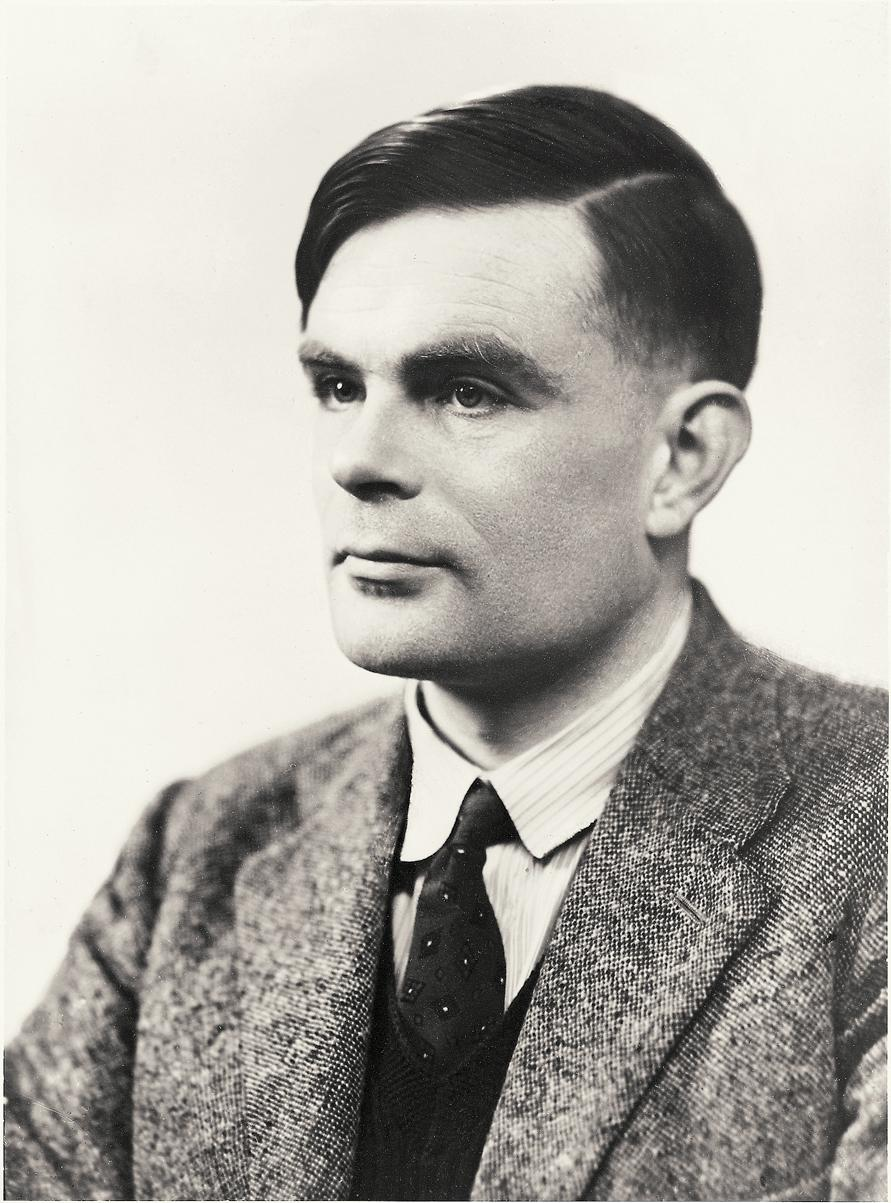
\includegraphics[width=0.8\linewidth]{pic/alan-turing.jpeg}
                \caption{Alan Turing}
            \end{figure}
            %\begin{figure}
            %    \centering
            %    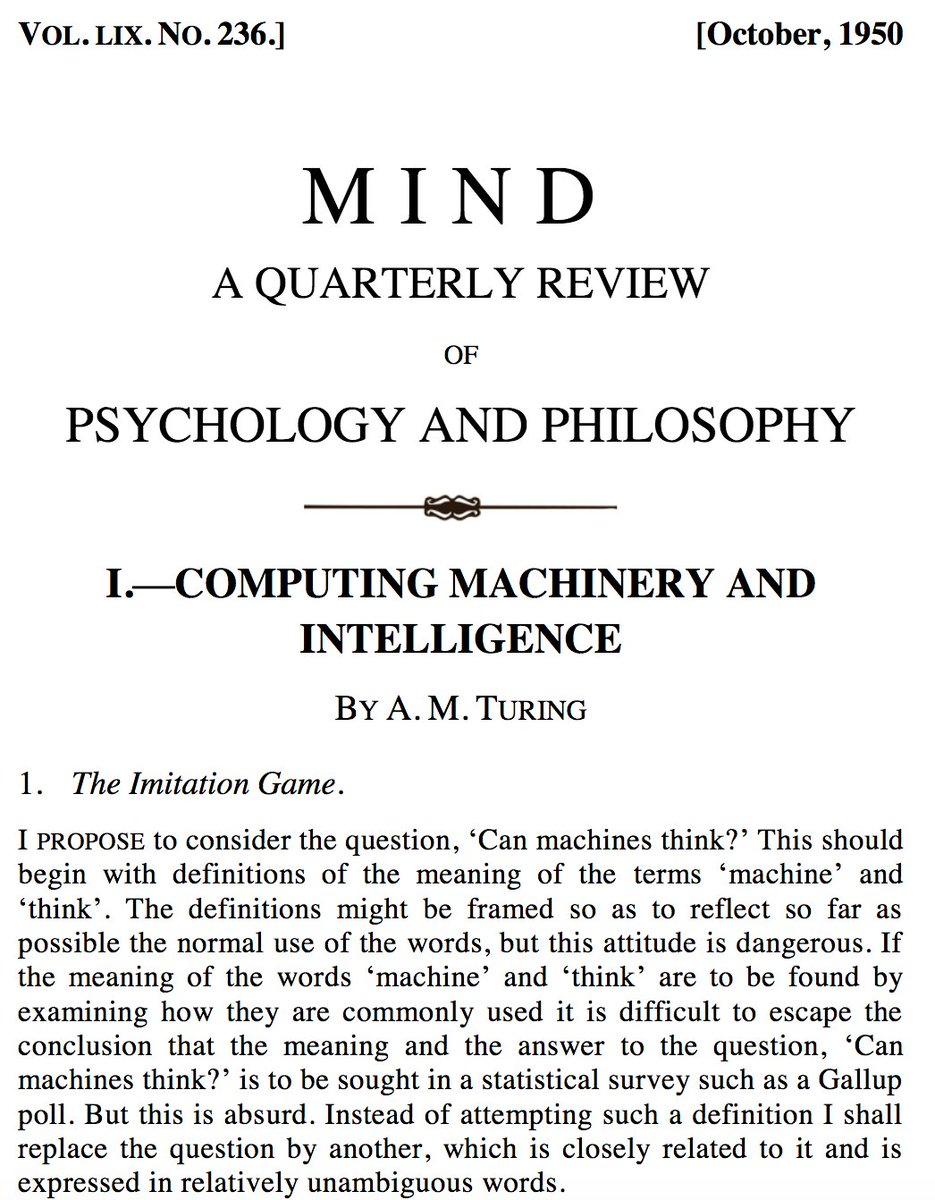
\includegraphics[width=0.6\linewidth]{pic/alan-turing-article.jpeg}
            %    \caption{"Computing Machinery and Intelligence" \textit{– Alan Turing (1950)}}
            %\end{figure}
    \end{columns}
\end{frame}

\subsubsection{Perceptron}

\begin{frame}{Machine Neuronale MIND 1024}
    \begin{columns}[T]
        \column{0.5\textwidth}
            \begin{figure}
                \centering
                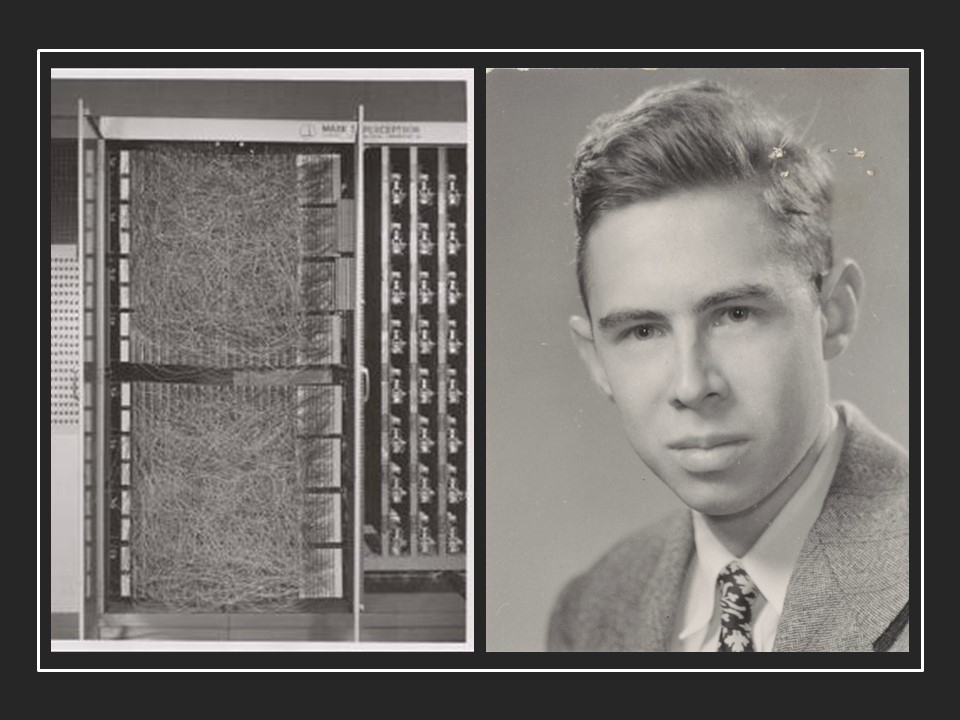
\includegraphics[width=0.65\linewidth]{pic/perceptron2.jpeg}
                \caption{Perceptron}
            \end{figure}
            \begin{figure}
                \centering
                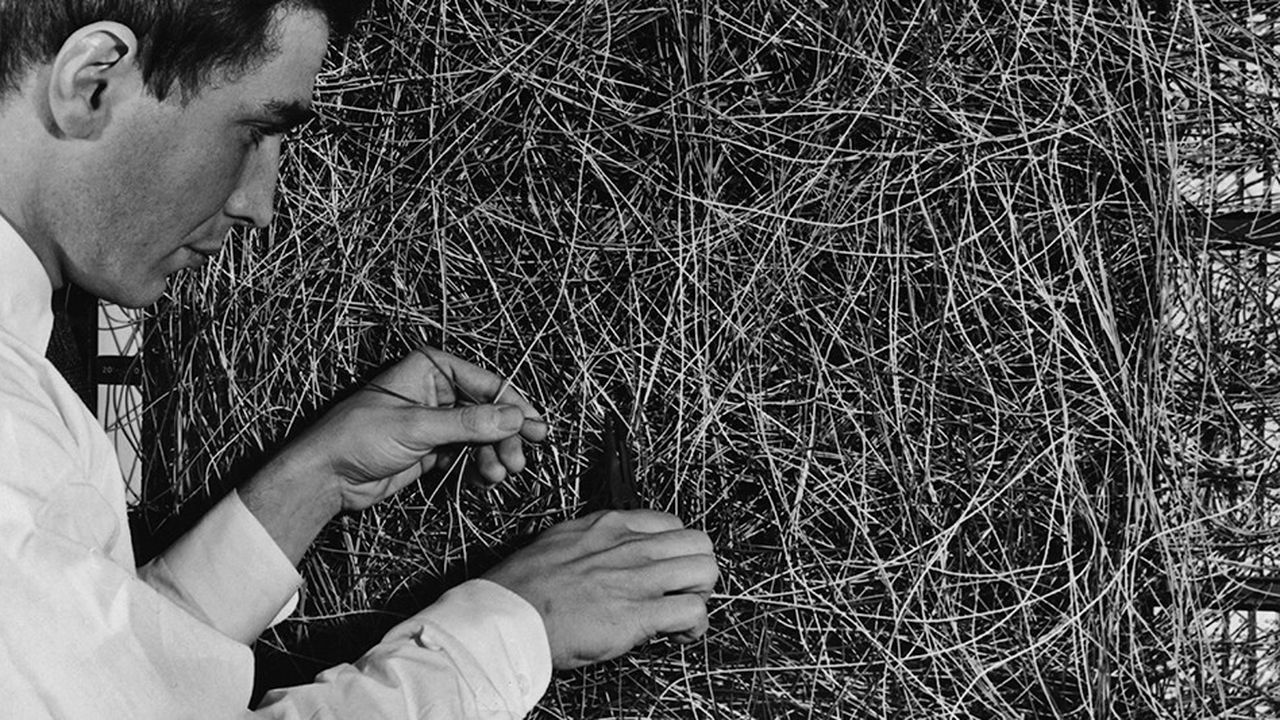
\includegraphics[width=0.6\linewidth]{pic/perceptron.jpeg}
                \caption{\textit{Frank Rosenblatt} et la machine}
            \end{figure}
        \column{0.5\textwidth}
            \begin{itemize}[<+-| alert@+>] % 当然,除了alert,手动在里面插 \pause 也行
                \item En 1958 : construction du \textit{Perceptron} par \textit{Frank Rosenblatt}.
                \item La machine visait à reconnaître des images.
                \item \textit{Warren McCulloch} et \textit{Walter Pitts} l'avait concpetualisée en 1943.
                \item Au début, \textit{Perceptron} avait du succès, mais cela se serait tari sous peu.
            \end{itemize}
    \end{columns}
\end{frame}

\subsubsection{John Hopfield}

\begin{frame}{Machine Neuronale MIND 1024}
    \begin{columns}[T]
        \column{0.5\textwidth}
            \begin{itemize}[<+-| alert@+>] % 当然,除了alert,手动在里面插 \pause 也行
                \item En 1982 \textit{John Hopfield} développe un réseau de neurones récurrents.
                \item Le MIND 1024 est implémenté trois ans plus tard à l'aide de ce type de réseau.
                \item De 1992 à 1994, la machine a servi d'un outil de recherche à Grenoble.
            \end{itemize}
            \begin{figure}
                \centering
                
\includegraphics[width=0.5\linewidth]{pic/aconit-logo.png}
                \caption{Perceptron}
            \end{figure}
        \column{0.5\textwidth}
            \begin{figure}
                \centering
                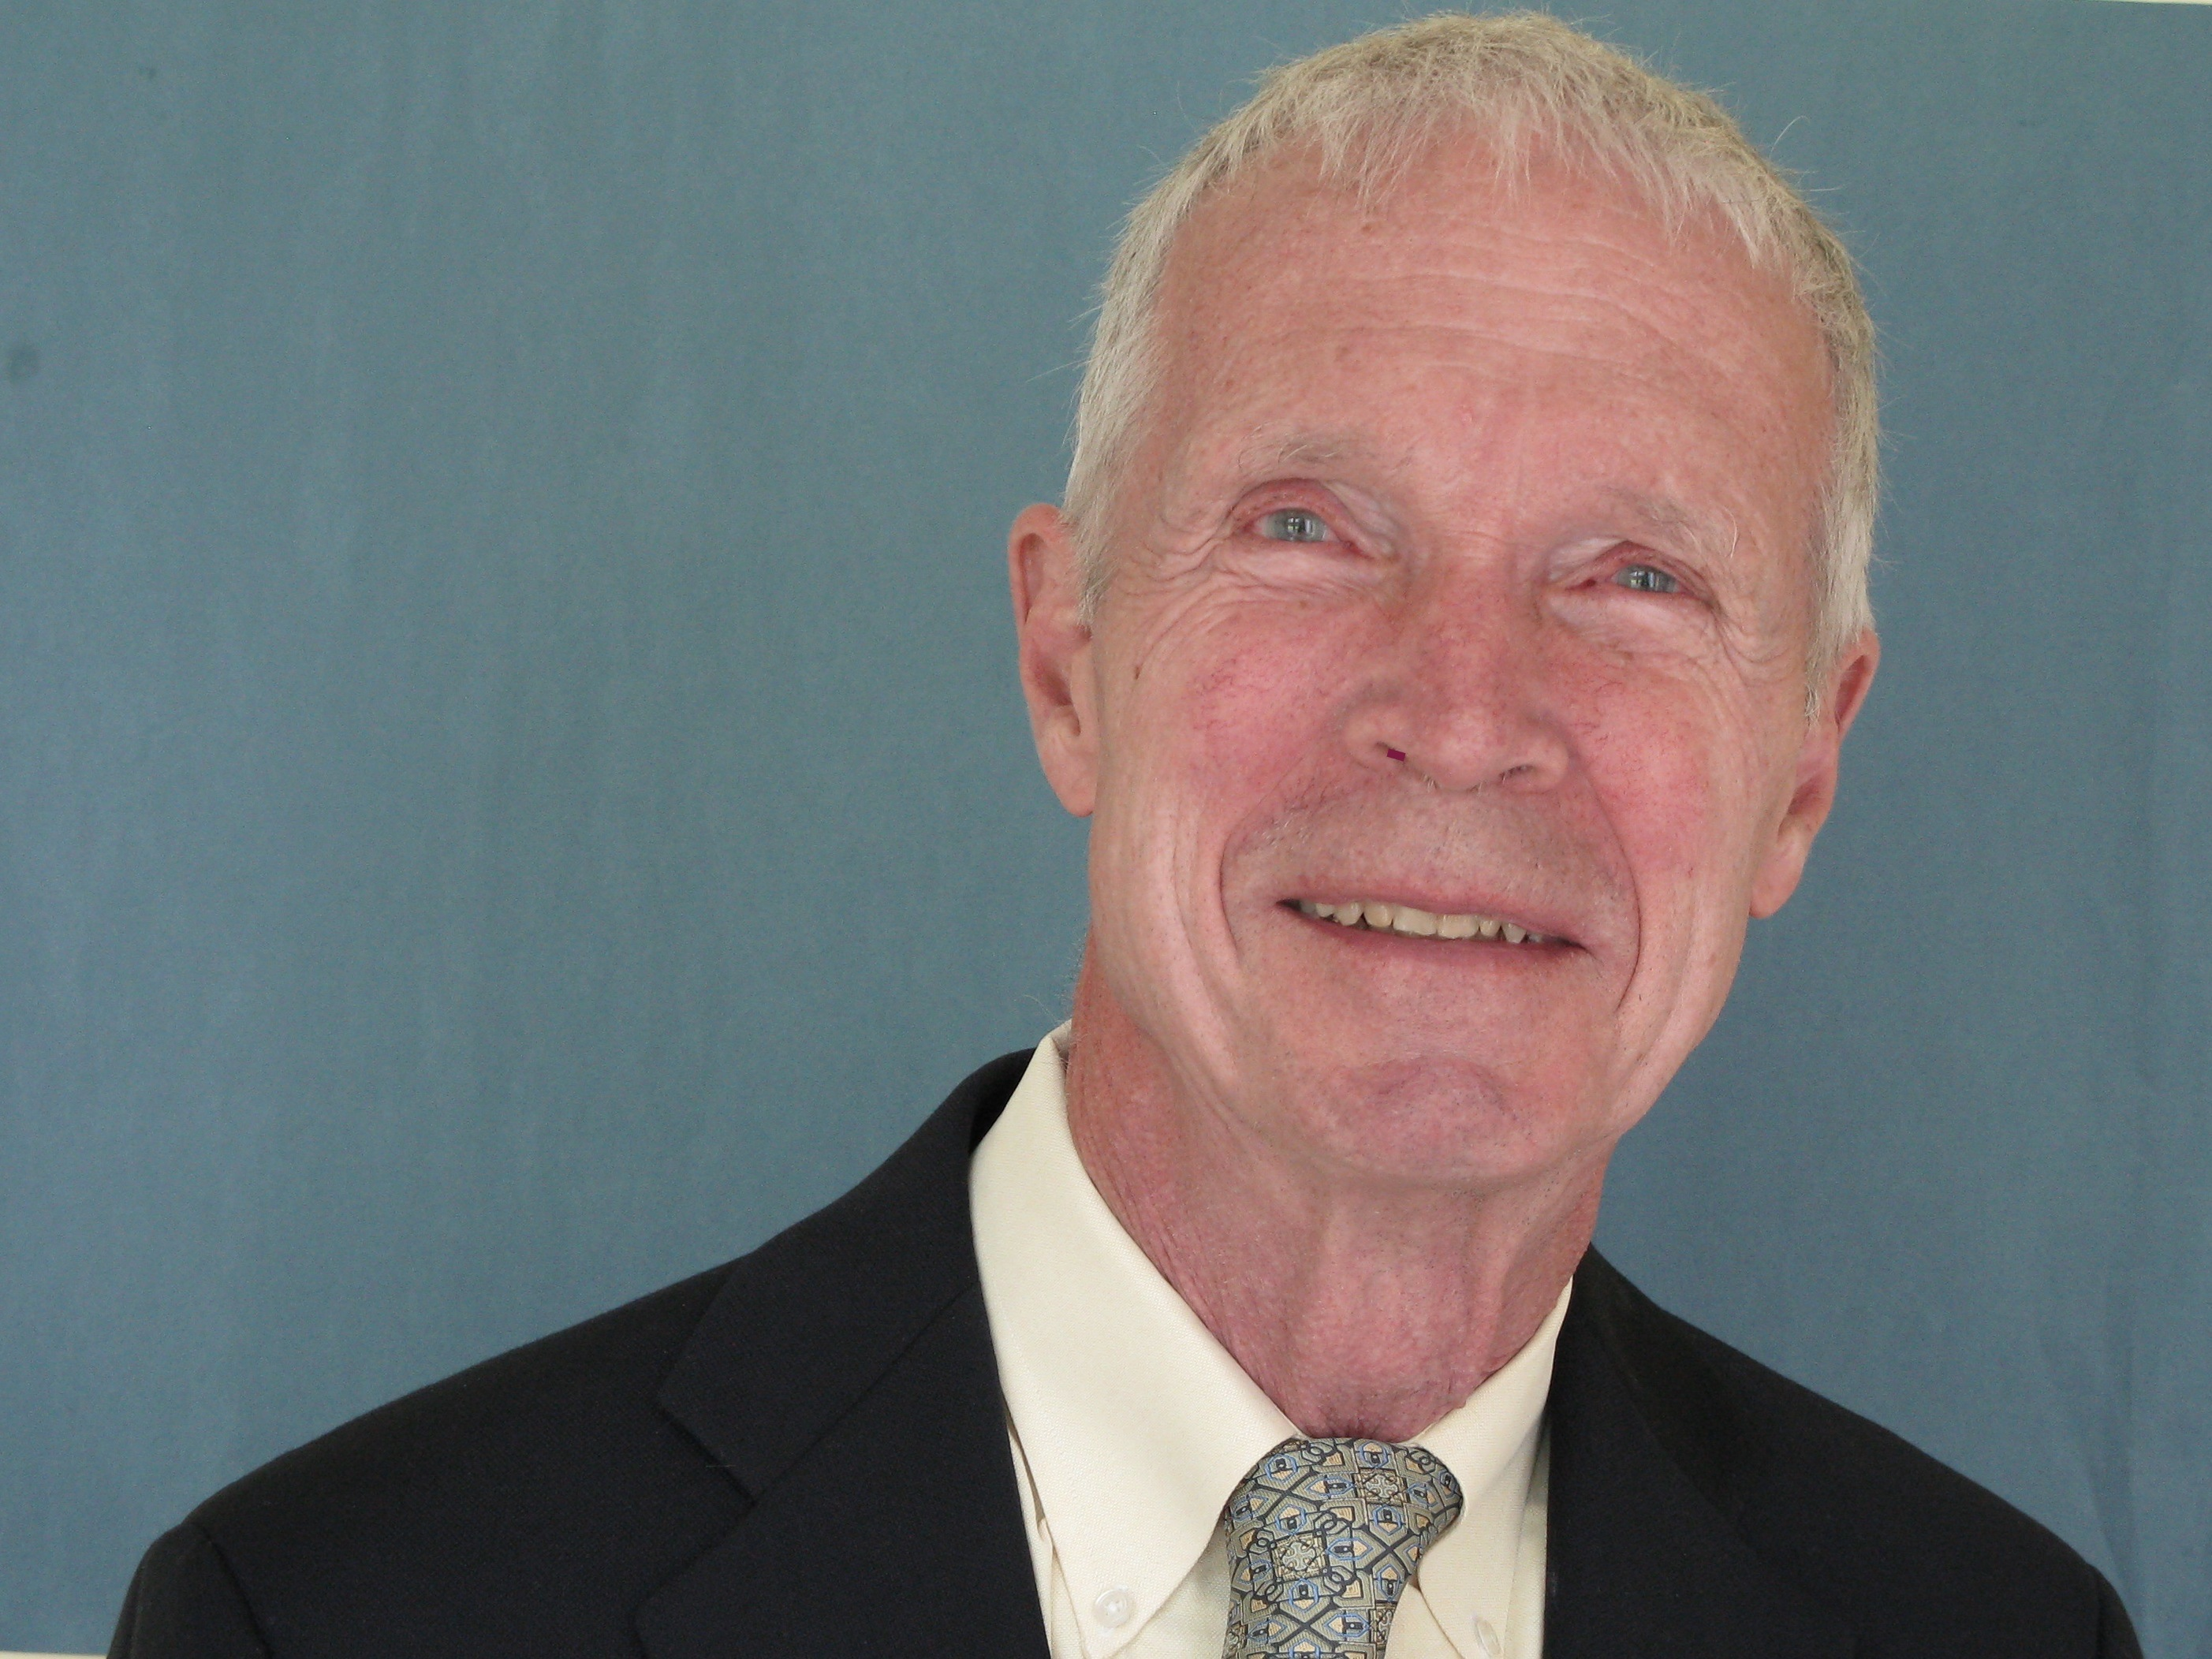
\includegraphics[width=0.55\linewidth]{pic/john-hopfield.jpeg}
                \caption{John Hopfield}
            \end{figure}
            \begin{figure}
                \centering
                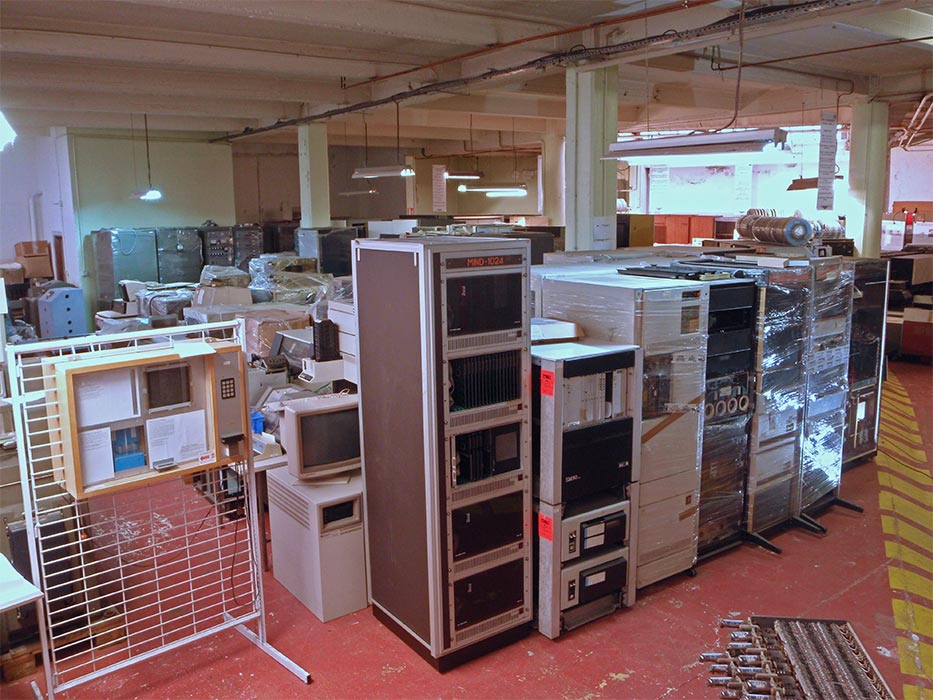
\includegraphics[width=0.6\linewidth]{pic/aconit1.jpeg}
                \caption{Le MIND 1024 à ACONIT}
            \end{figure}
    \end{columns}
\end{frame}

\section{Réseau de Hopfield plus en profondeur}

\subsection{En quoi ça consiste ?}

\begin{frame}{Machine Neuronale MIND 1024}
    \begin{itemize}[<+-| alert@+>] % 当然,除了alert,手动在里面插 \pause 也行
        \item Réseau de Hopfield : composé de neurones tous interconnectés.
    \end{itemize}
    \begin{columns}[T]
        \column{0.50\textwidth}
            \begin{figure}
                \centering
                \includegraphics[width=1.0\linewidth]{pic/Réseau-Neuronale-2.png}
                \caption{Réseau de 5 neurones}
            \end{figure}
        \column{0.50\textwidth}
            \begin{figure}
                \centering
                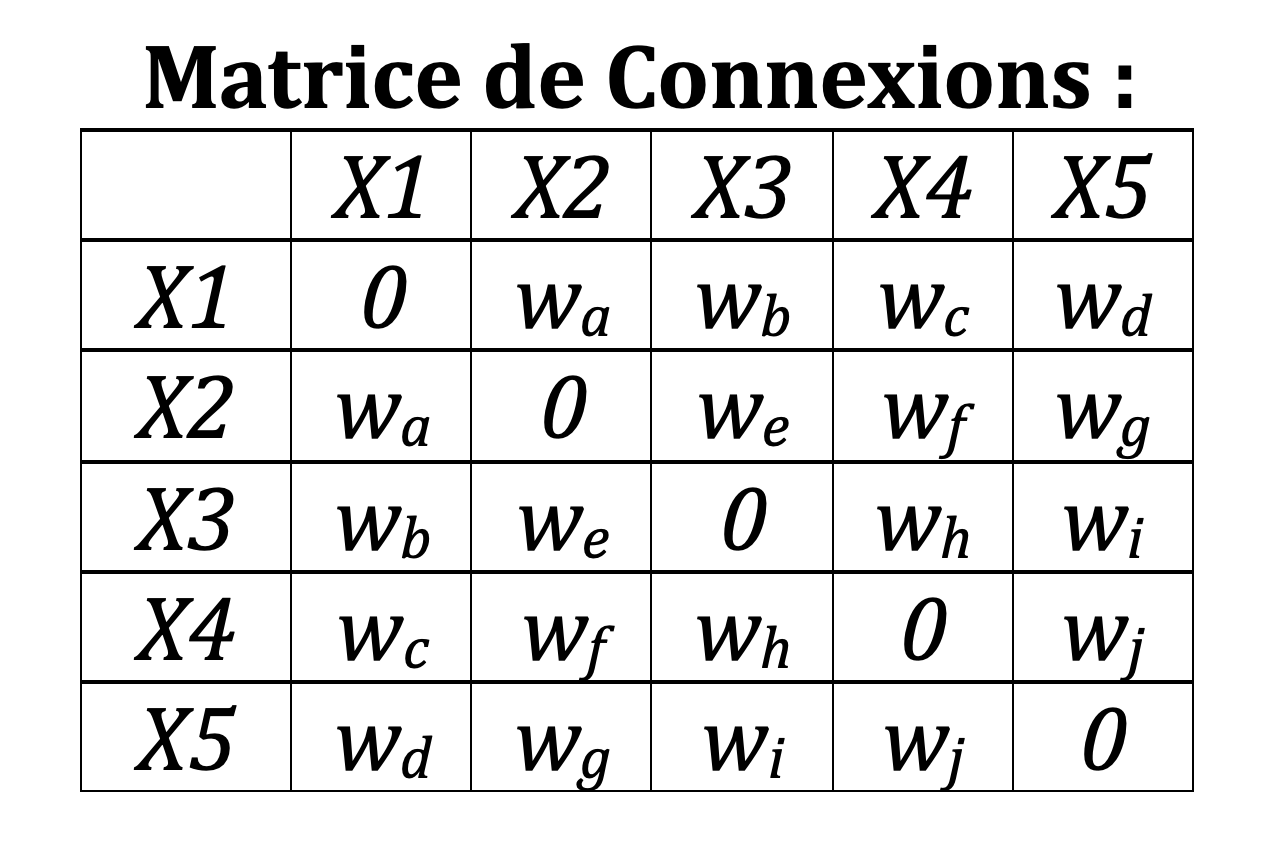
\includegraphics[width=1.0\linewidth]{pic/Matrice-de-connexions.png}
            \end{figure}
            \[w_{ij} = w_{ji} \in \{-1, 1\}, w_{ii} = 0\]
    \end{columns}
\end{frame}

\subsection{Règle de mise à jour}

\begin{frame}{Machine Neuronale MIND 1024}
    \begin{itemize}[<+-| alert@+>] % 当然,除了alert,手动在里面插 \pause 也行
        \item Règle de mise à jour des états $x_i$ :
        \item $
                x_i \leftarrow
                \begin{cases}
                +1,& \text{si} \sum_j w_{ij} x_j \geq \theta_i,\\
                -1,& \text{sinon}
                \end{cases}
              $
        \item Effet de cette règle :
            \begin{itemize}[<+-| alert@+>] % 当然,除了alert,手动在里面插 \pause 也行
                \item Si $w_{ij} > 0$, $x_i$ et $x_j$ vont \textbf{converger}.
                \item Si $w_{ij} < 0$, $x_i$ et $x_j$ vont \textbf{diverger}.
            \end{itemize}
    \end{itemize}
\end{frame}

\subsection{Petit exemple}

\begin{frame}{Machine Neuronale MIND 1024}
    \begin{itemize}[<+-| alert@+>] % 当然,除了alert,手动在里面插 \pause 也行
        \item Petit Exemple :
        \item On a un motif, (c'est-à-dire un ensemble d'états).
        \item On veut que le réseau puisse retrouver ce motif.
        \item Alors, on peut fixer les valeurs des poids des connexions telles que :
        \begin{itemize}[<+-| alert@+>] % 当然,除了alert,手动在里面插 \pause 也行
            \item $w_{ij} > 0$ pour $x_i = x_j$
            \item $w_{ij} < 0$ pour $x_i \neq x_j$
        \end{itemize}
    \end{itemize}
\end{frame}

\begin{frame}{Machine Neuronale MIND 1024}
    \begin{figure}
        \centering
        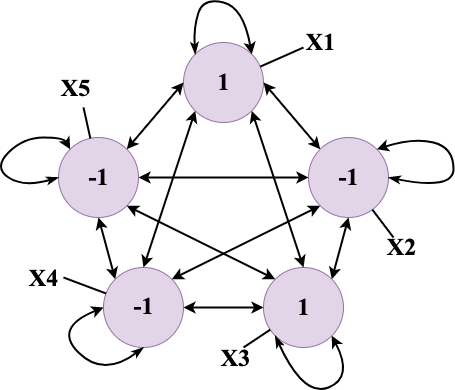
\includegraphics[width=0.5\linewidth]{pic/network1.png}
    \end{figure}
\end{frame}

\begin{frame}{Machine Neuronale MIND 1024}
    \begin{columns}[T]
        \column{0.5\textwidth}
        \begin{figure}
            \centering
            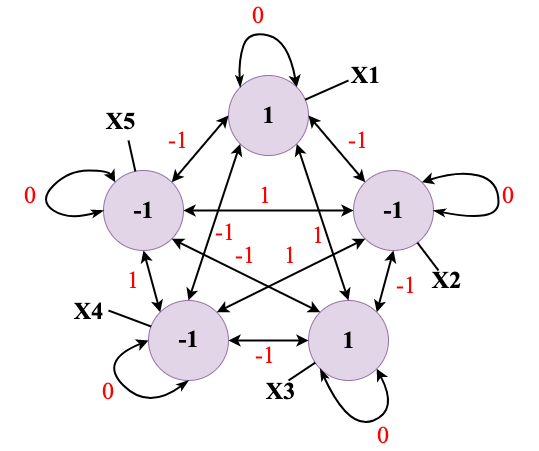
\includegraphics[width=1.25\linewidth]{pic/network2.png}
        \end{figure}
        \column{0.5\textwidth}
            \begin{figure}
            \centering
            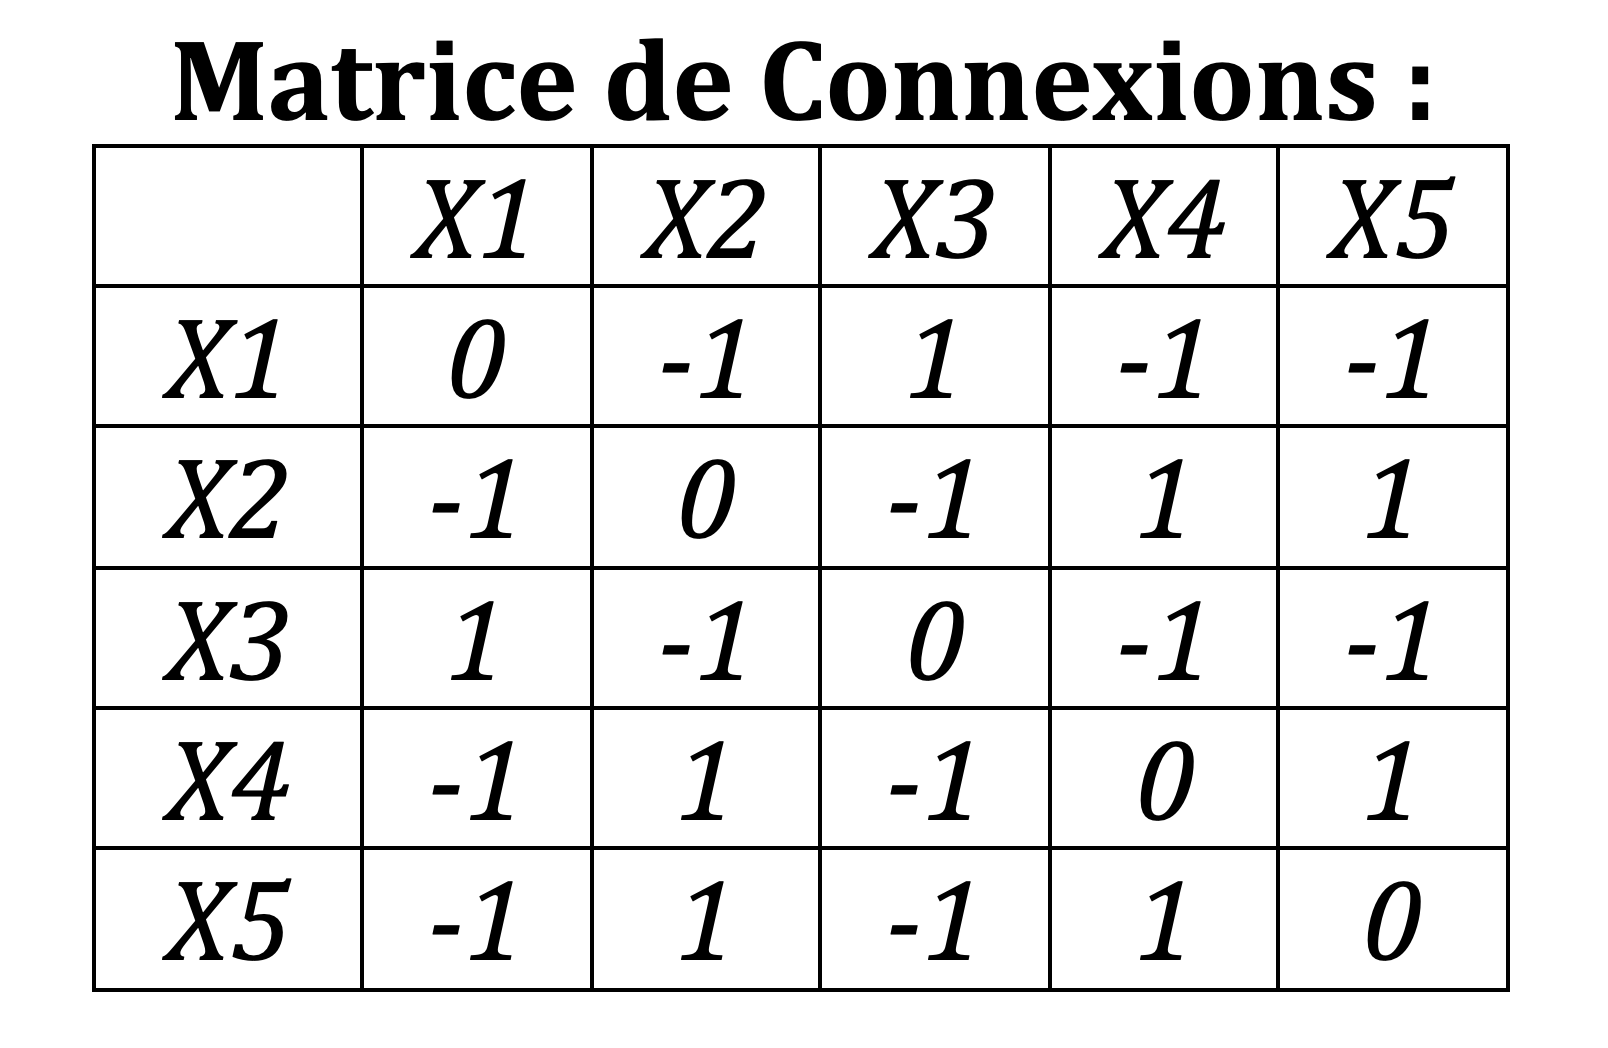
\includegraphics[width=0.8\linewidth]{pic/matrix.png}
            \end{figure}
    \end{columns}
\end{frame}

\begin{frame}{Machine Neuronale MIND 1024}
    \begin{columns}[T]
        \column{0.4\textwidth}
            \begin{itemize}[<+-| alert@+>] % 当然,除了alert,手动在里面插 \pause 也行
                \item Après avoir décidé les poids, on peut changer la valeur d'un état...
            \end{itemize}
            \begin{figure}
                \centering
                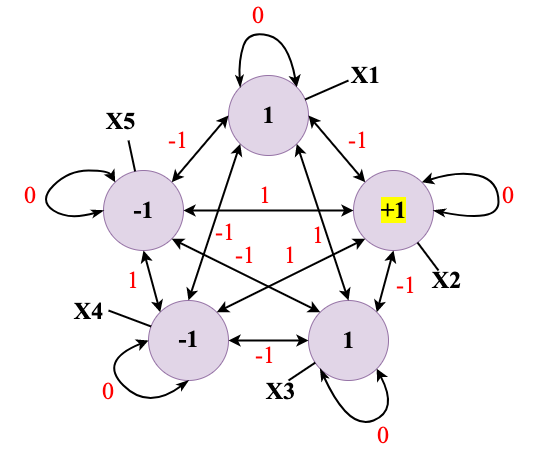
\includegraphics[width=1.25\linewidth]{pic/network3.png}
            \end{figure}
        \column{0.6\textwidth}
            \begin{itemize}[<+-| alert@+>] % 当然,除了alert,手动在里面插 \pause 也行
                \item ..puis, on peut appliquer la règle de tout à l'heure :
                \item $
                        x_i \leftarrow
                        \begin{cases}
                        +1,& \text{si} \sum_j w_{ij} x_j \geq \theta_i,\\
                        -1,& \text{sinon}
                        \end{cases}
                    $
                \item En théorie, le réseau corrigera l'état différent afin de retourner au motif original.
                \item La machine aura retrouvé le motif \og dans sa mémoire \fg{}.
            \end{itemize}
    \end{columns}
\end{frame}

\subsection{Règle de Hebb}

\begin{frame}{Machine Neuronale MIND 1024}
    \begin{itemize}[<+-| alert@+>] % 当然,除了alert,手动在里面插 \pause 也行
        \item Règle de Hebb, introduite par \textit{Donald Hebb} en 1949 :
        \item Soit $n$ la taille de l'ensemble de configurations cibles du réseau $\{x_1, ..., x_n\}$,
        \item $w_{ij} = \frac{1}{n}\sum_{\mu=1}^{n}x_{i}^{\mu}x_{j}^{\mu}$, où $x_{i}^{\mu}$ représente bit $i$ de motif $\mu$.
        \item $w_{ij} = 0$.
        \item Effet de cette règle :
            \begin{itemize}[<+-| alert@+>] % 当然,除了alert,手动在里面插 \pause 也行
                \item C'est le calcul de l'activation moyenne entre deux neurones voisins.
                \item Si les bits qui correspondent aux neurones $i$ et $j$ sont égals dans motif $\mu$, alors le produit $x_{i}^{\mu}x_{j}^{\mu}$ sera positif. Par conséquent, le poids $w_{ij}$ tend à être positif et donc les valeurs de $i$ et $j$ tendent à être égales.
                \item Si les bits qui correspondent aux neurones $i$ et $j$ sont différents dans motif $\mu$, c'est l'inverse.
            \end{itemize}
    \end{itemize}
\end{frame}

\section{Simulateur}

\subsection{Code}

\begin{frame}{Machine Neuronale MIND 1024}
    \begin{itemize}[<+-| alert@+>] % 当然,除了alert,手动在里面插 \pause 也行
        \item Pour démontrer l'utilité du MIND 1024, il faut un simulateur d'un réseau de Hopfield.
        \item Je me suis procuré du code de base sur GitHub. Utilisateur : Alex Nichol (\textit{https://github.com/unixpickle}).
        \item Il s'agit d'une application qui correspond un dessin donné à un dessin mémorisé.
        \item L'application est implémentée avec \textit{Javascript}.
        \begin{figure}
            \centering
            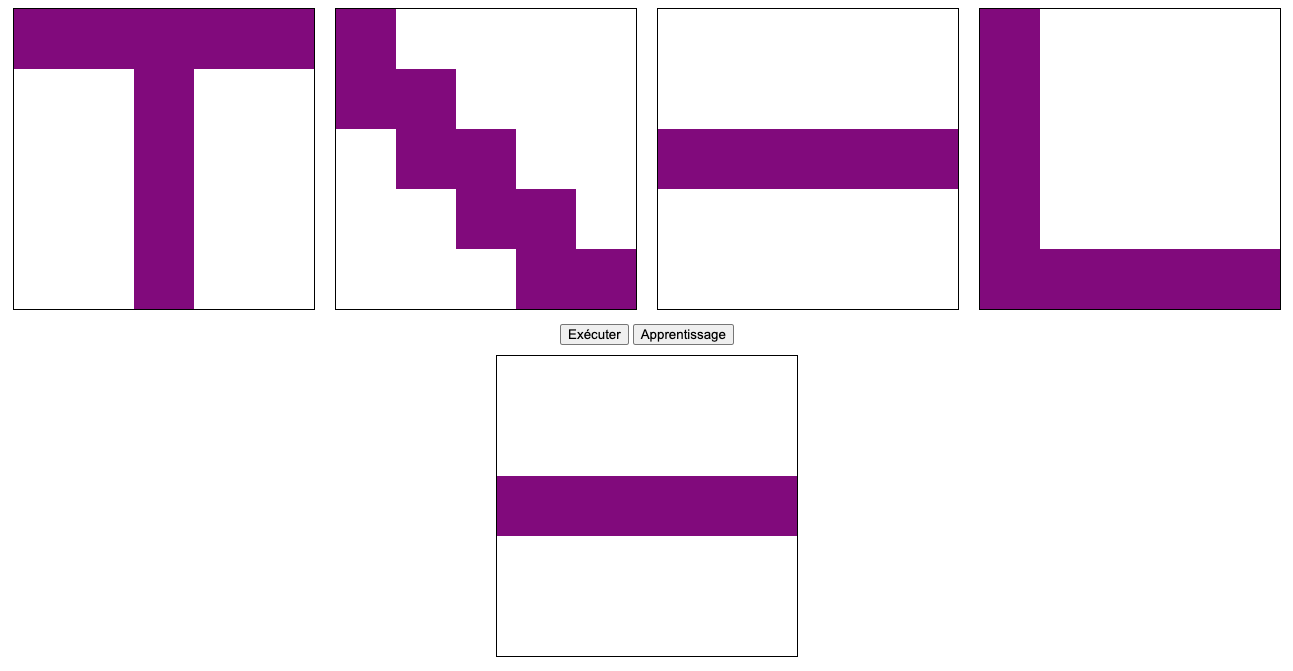
\includegraphics[width=0.7\linewidth]{pic/app1.png}
        \end{figure}
    \end{itemize}
\end{frame}

\begin{frame}{Machine Neuronale MIND 1024}
    Fonction 'convergeRandomNode' (calcul d'un nouvel état aléatoire) :
    \begin{figure}
        \centering
        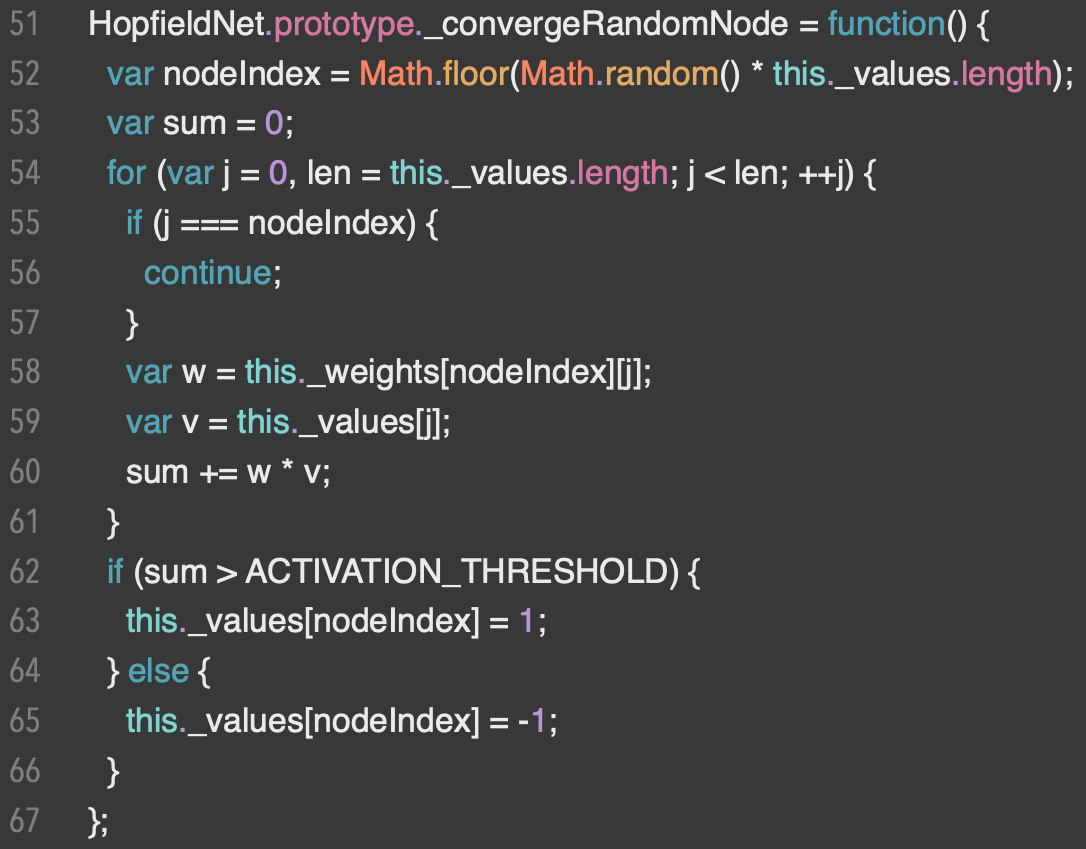
\includegraphics[width=0.7\linewidth]{pic/alg1.png}
    \end{figure}
\end{frame}  

\begin{frame}{Machine Neuronale MIND 1024}
    \begin{itemize}[<+-| alert@+>] % 当然,除了alert,手动在里面插 \pause 也行
        \item La fonction au-dessus converge un neurone aléatoire.
        \item Elle correspond à la règle que l'on a vue :
        \item $
                        x_i \leftarrow
                        \begin{cases}
                        +1,& \text{si} \sum_j w_{ij} x_j \geq \theta_i,\\
                        -1,& \text{sinon}
                        \end{cases}
                    $
        \item En fait, il existe 2 types de mise à jour de l'état :
            \begin{itemize}[<+-| alert@+>] % 当然,除了alert,手动在里面插 \pause 也行
                \item \textbf{Asynchrone :} le cacul de nouveaux états se fait \textit{un état à la fois}.
                \item \textbf{Synchrone :} la mise à jour prend en compte tous les états simultanément. Cette méthode nécissite un horloge pour maintenir la synchronisation.
            \end{itemize}
    \end{itemize}
\end{frame}

\begin{frame}{Machine Neuronale MIND 1024}
    Fonction 'train' (apprentissage) :
    \begin{figure}
        \centering
        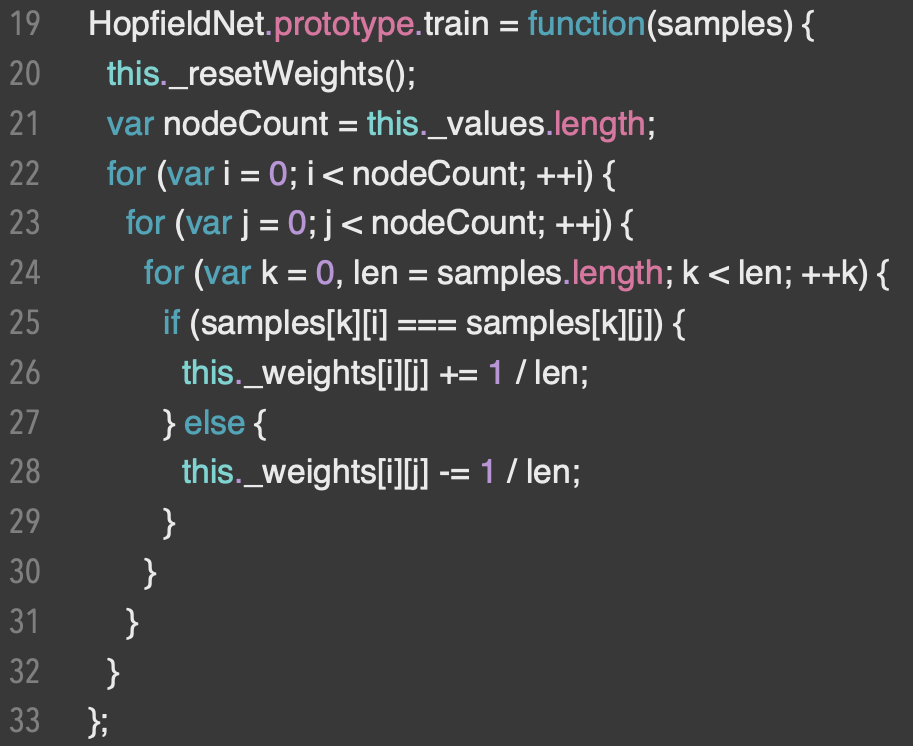
\includegraphics[width=0.7\linewidth]{pic/alg2.png}
    \end{figure}
\end{frame}  

\begin{frame}{Machine Neuronale MIND 1024}
    \begin{itemize}[<+-| alert@+>] % 当然,除了alert,手动在里面插 \pause 也行
        \item La fonction au-dessus fixe les valeurs des poids des connexions à partir des dessins d'entrée, (les échantillons).
        \item Elle correspond à la règle de Hebb :
        \item $w_{ij} = \frac{1}{n}\sum_{\mu=1}^{n}x_{i}^{\mu}x_{j}^{\mu}$
        \item Ici :
            \begin{itemize}[<+-| alert@+>] % 当然,除了alert,手动在里面插 \pause 也行
                \item Le variable $len$ correspond à la taille de l'ensemble d'échantillons $n$.
                \item Le variable $k$ correspond à un échantillon $\mu$.
            \end{itemize}
    \end{itemize}
\end{frame}

\subsection{Code QR}

\begin{frame}{Machine Neuronale MIND 1024}
    \begin{itemize}[<+-| alert@+>] % 当然,除了alert,手动在里面插 \pause 也行
        \item Une image de taille $n^2$ produit un réseau de $n^2$ neurones tous interconnectés.
        \item Le MIND 1024 possède 1024 et donc la taille maximale d'une image que l'on lui aurait pu fournir est de $n^2 = 1024$, $\therefore n = \sqrt{1024} = 32$.
        \item Je voudrais essayer des codes QR comme échantillons.
        \item Il suffit donc d'ajuster le variable 'PICTURE\_SIZE' :
        \begin{figure}
            \centering
            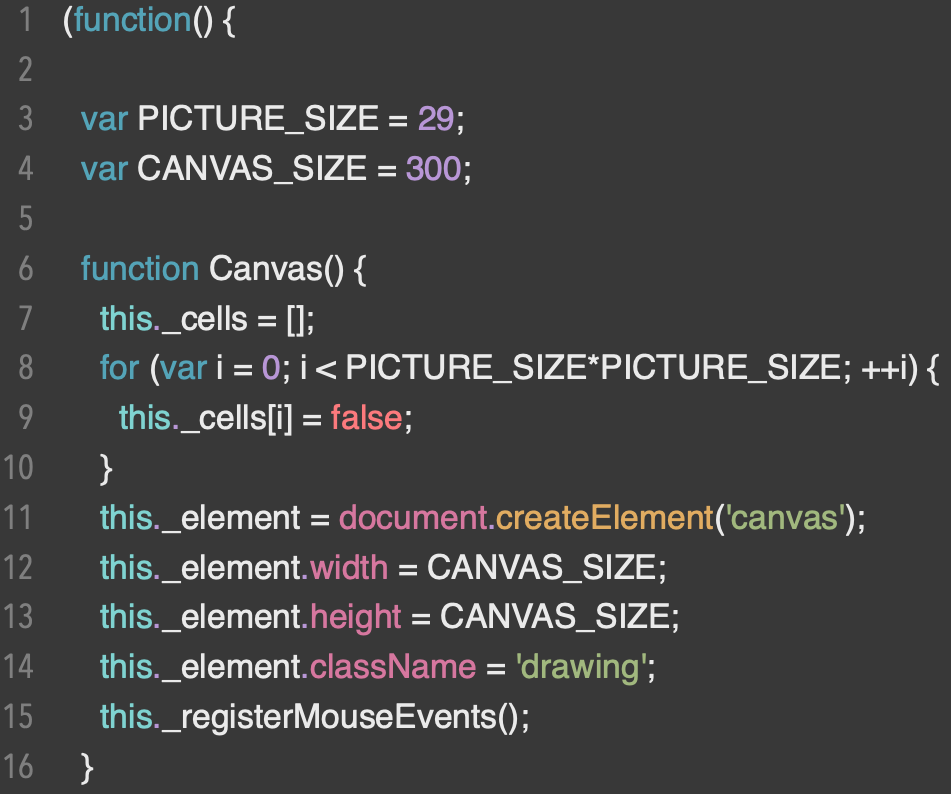
\includegraphics[width=0.38\linewidth]{pic/alg3.png}
        \end{figure}
    \end{itemize}
\end{frame}

\begin{frame}{Machine Neuronale MIND 1024}
    \begin{itemize}[<+-| alert@+>] % 当然,除了alert,手动在里面插 \pause 也行
        \item On peut avoir un code QR de taille $33*33$ pixels, mais cela aurait créé un réseau avec trop de neurones.
        \item Alors, un code QR de taille $29*29$ pixels est aussi possible et donc j'en crée 3.
    \end{itemize}
\end{frame}

\begin{frame}{Machine Neuronale MIND 1024}
    \begin{itemize}[<+-| alert@+>] % 当然,除了alert,手动在里面插 \pause 也行
        \item Pour le premier, je génère un code QR à partir d'une phrase courte :
        \item \og Qu'ils mangent de la brioche !\fg{}
        \item Il sert d'un échantillon.
        \begin{figure}
            \centering
            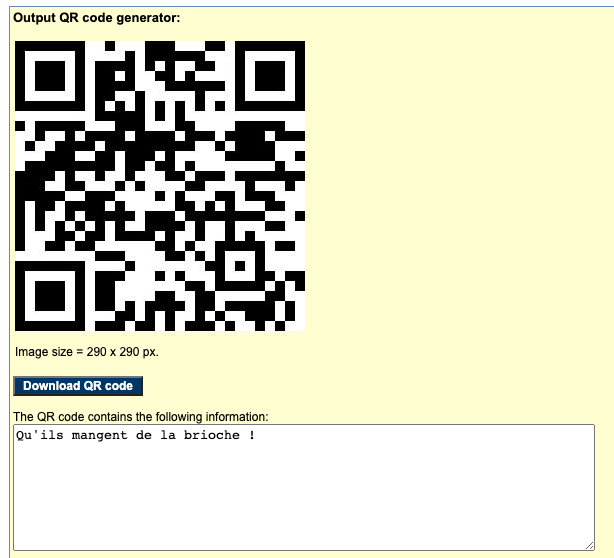
\includegraphics[width=0.5\linewidth]{pic/qr1.png}
            \caption{Code QR 1 : Échantillon 1}
        \end{figure}
    \end{itemize}
\end{frame}

\begin{frame}{Machine Neuronale MIND 1024}
    \begin{itemize}[<+-| alert@+>] % 当然,除了alert,手动在里面插 \pause 也行
        \item Pour le second, je génère un code QR à partir d'une phrase courte similaire :
        \item \og Qu'ils mangent du gâteau !\fg{}
        \item Il sert aussi d'un échantillon.
        \begin{figure}
            \centering
            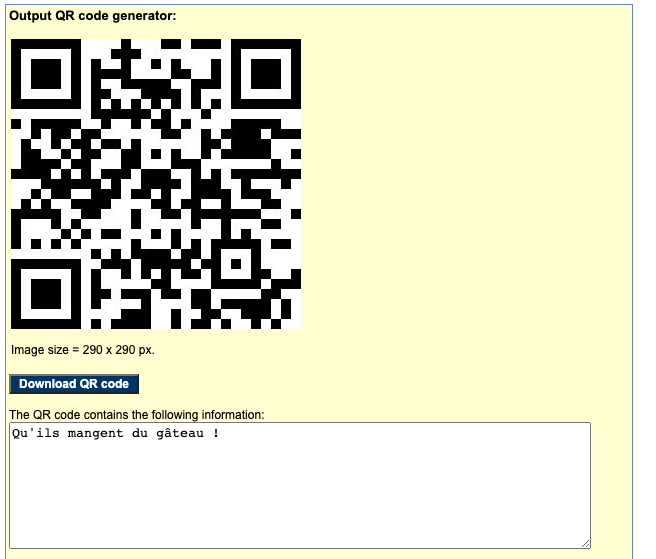
\includegraphics[width=0.5\linewidth]{pic/qr2.png}
            \caption{Code QR 2 : Échantillon 2}
        \end{figure}
    \end{itemize}
\end{frame}

\begin{frame}{Machine Neuronale MIND 1024}
    \begin{itemize}[<+-| alert@+>] % 当然,除了alert,手动在里面插 \pause 也行
        \item Pour le troisième, je génère un code QR à partir d'une phrase courte similaire à la première phrase :
        \item \og Qu'ils mangent de la brique !\fg{}
        \item Il sert de la nouvelle image.
        %\item \textit{(Le sens est un peu bizarre, mais je voulais que ce soit presque pareil que la première)}.
        \begin{figure}
            \centering
            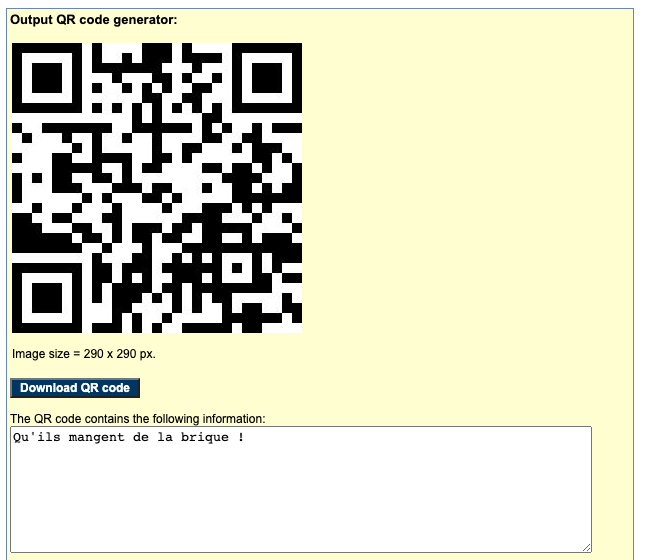
\includegraphics[width=0.5\linewidth]{pic/qr3.png}
            \caption{Code QR 3 : Nouvelle Image}
        \end{figure}
    \end{itemize}
\end{frame}

\begin{frame}{Machine Neuronale MIND 1024}
    Alors, je teste l'application avec ces trois codes QR...
    \begin{figure}
        \centering
        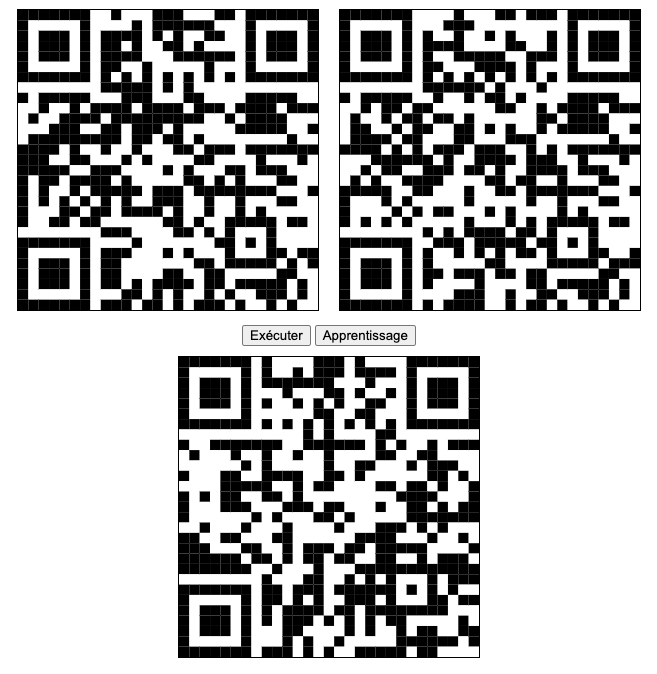
\includegraphics[width=0.6\linewidth]{pic/qrinput.png}
        \caption{Avant Exécution}
    \end{figure}
\end{frame}

\begin{frame}{Machine Neuronale MIND 1024}
    ...et le code QR le plus similaire, (le premier), est bien retrouvé !
    \begin{figure}
        \centering
        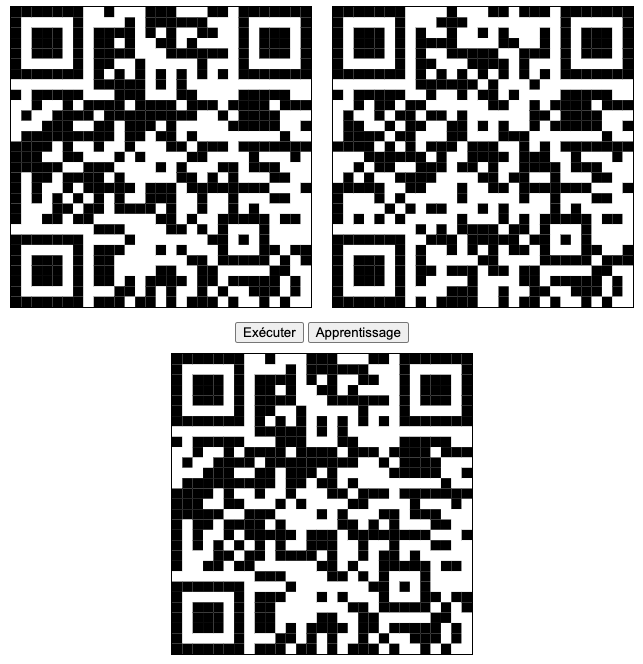
\includegraphics[width=0.6\linewidth]{pic/qroutput.png}
        \caption{Après Exécution}
    \end{figure}
\end{frame}

\iffalse
\subsection{Beamer主题分类}

\begin{frame}
    \begin{itemize}
        \item 有一些 \LaTeX{} 自带的
        \item 有一些Tsinghua的
        \item 本模板来源自THU Beamer Theme
        \item 但是最初的 \href{http://far.tooold.cn/post/latex/beamertsinghua}{\color{purple}{link}} \cite{origin}已经失效了
        \item 这是原作者在16-17年做的一些ppt:\href{https://github.com/Trinkle23897/oi_slides}{\color{blue}{戳我}}
    \end{itemize}
\end{frame}

\subsection{美化主题}

\begin{frame}{这一份主题与原始的THU Beamer Theme区别在于}
    \begin{itemize}
        \item 顶栏的小点变成一行而不是多行
        \item 中文采用楷书
        \item 修改了主题色为南邮校徽颜色
        \item 参考文献格式按照毕设标准进行了修改
        \item 更多该模板的功能可以参考 \url{https://www.latexstudio.net/archives/4051.html}
        \item 下面列举出了一些Beamer的用法,部分节选自 \url{https://tuna.moe/event/2018/latex/}
    \end{itemize}
\end{frame}

\subsection{如何更好地做Beamer}

\begin{frame}{Why Beamer}
    \begin{itemize}
        \item \LaTeX 广泛用于学术界,期刊会议论文模板
    \end{itemize}
    \begin{table}[h]
        \centering
        \begin{tabular}{c|c}
            Microsoft\textsuperscript{\textregistered}  Word & \LaTeX \\
            \hline
            文字处理工具 & 专业排版软件 \\
            容易上手,简单直观 & 容易上手 \\
            所见即所得 & 所见即所想,所想即所得 \\
            高级功能不易掌握 & 进阶难,但一般用不到 \\
            处理长文档需要丰富经验 & 和短文档处理基本无异 \\
            花费大量时间调格式 & 无需担心格式,专心作者内容 \\
            公式排版差强人意 & 尤其擅长公式排版 \\
            二进制格式,兼容性差 & 文本文件,易读、稳定 \\
            付费商业许可 & 自由免费使用 \\
        \end{tabular}
    \end{table}
\end{frame}

\begin{frame}{排版举例}
    \begin{exampleblock}{无编号公式} % 加 * 
        \begin{equation*}
            J(\theta) = \mathbb{E}_{\pi_\theta}[G_t] = \sum_{s\in\mathcal{S}} d^\pi (s)V^\pi(s)=\sum_{s\in\mathcal{S}} d^\pi(s)\sum_{a\in\mathcal{A}}\pi_\theta(a|s)Q^\pi(s,a)
        \end{equation*}
    \end{exampleblock}
    \begin{exampleblock}{多行多列公式\footnote{如果公式中有文字出现,请用 $\backslash$mathrm\{\} 或者 $\backslash$text\{\} 包含,不然就会变成 $clip$,在公式里看起来比 $\mathrm{clip}$ 丑非常多。}}
        % 使用 & 分隔
        \begin{align}
            Q_\mathrm{target}&=r+\gamma Q^\pi(s^\prime, \pi_\theta(s^\prime)+\epsilon)\\
            \epsilon&\sim\mathrm{clip}(\mathcal{N}(0, \sigma), -c, c)\nonumber
        \end{align}
    \end{exampleblock}
\end{frame}

\begin{frame}
    \begin{exampleblock}{编号多行公式}
        % Taken from Mathmode.tex
        \begin{multline}
            A=\lim_{n\rightarrow\infty}\Delta x\left(a^{2}+\left(a^{2}+2a\Delta x+\left(\Delta x\right)^{2}\right)\right.\label{eq:reset}\\
            +\left(a^{2}+2\cdot2a\Delta x+2^{2}\left(\Delta x\right)^{2}\right)\\
            +\left(a^{2}+2\cdot3a\Delta x+3^{2}\left(\Delta x\right)^{2}\right)\\
            +\ldots\\
            \left.+\left(a^{2}+2\cdot(n-1)a\Delta x+(n-1)^{2}\left(\Delta x\right)^{2}\right)\right)\\
            =\frac{1}{3}\left(b^{3}-a^{3}\right)
        \end{multline}
    \end{exampleblock}
\end{frame}

\begin{frame}{图形与分栏}
    % From thuthesis user guide.
    \begin{minipage}[c]{0.3\linewidth}
        \psset{unit=0.8cm}
        \begin{pspicture}(-1.75,-3)(3.25,4)
            \psline[linewidth=0.25pt](0,0)(0,4)
            \rput[tl]{0}(0.2,2){$\vec e_z$}
            \rput[tr]{0}(-0.9,1.4){$\vec e$}
            \rput[tl]{0}(2.8,-1.1){$\vec C_{ptm{ext}}$}
            \rput[br]{0}(-0.3,2.1){$\theta$}
            \rput{25}(0,0){%
            \psframe[fillstyle=solid,fillcolor=lightgray,linewidth=.8pt](-0.1,-3.2)(0.1,0)}
            \rput{25}(0,0){%
            \psellipse[fillstyle=solid,fillcolor=yellow,linewidth=3pt](0,0)(1.5,0.5)}
            \rput{25}(0,0){%
            \psframe[fillstyle=solid,fillcolor=lightgray,linewidth=.8pt](-0.1,0)(0.1,3.2)}
            \rput{25}(0,0){\psline[linecolor=red,linewidth=1.5pt]{->}(0,0)(0.,2)}
%           \psRotation{0}(0,3.5){$\dot\phi$}
%           \psRotation{25}(-1.2,2.6){$\dot\psi$}
            \psline[linecolor=red,linewidth=1.25pt]{->}(0,0)(0,2)
            \psline[linecolor=red,linewidth=1.25pt]{->}(0,0)(3,-1)
            \psline[linecolor=red,linewidth=1.25pt]{->}(0,0)(2.85,-0.95)
            \psarc{->}{2.1}{90}{112.5}
            \rput[bl](.1,.01){C}
        \end{pspicture}
    \end{minipage}\hspace{1cm}
    \begin{minipage}{0.5\linewidth}
        \medskip
        %\hspace{2cm}
        \begin{figure}[h]
            \centering
            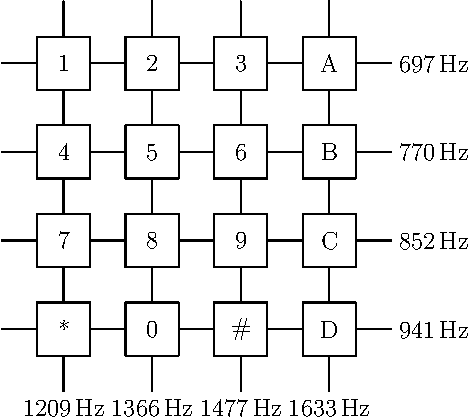
\includegraphics[height=.4\textheight]{pic/dtmf.pdf}
        \end{figure}
    \end{minipage}
\end{frame}

\begin{frame}[fragile]{\LaTeX{} 常用命令}
    \begin{exampleblock}{命令}
        \centering
        \footnotesize
        \begin{tabular}{llll}
            \cmd{chapter} & \cmd{section} & \cmd{subsection} & \cmd{paragraph} \\
            章 & 节 & 小节 & 带题头段落 \\\hline
            \cmd{centering} & \cmd{emph} & \cmd{verb} & \cmd{url} \\
            居中对齐 & 强调 & 原样输出 & 超链接 \\\hline
            \cmd{footnote} & \cmd{item} & \cmd{caption} & \cmd{includegraphics} \\
            脚注 & 列表条目 & 标题 & 插入图片 \\\hline
            \cmd{label} & \cmd{cite} & \cmd{ref} \\
            标号 & 引用参考文献 & 引用图表公式等\\\hline
        \end{tabular}
    \end{exampleblock}
    \begin{exampleblock}{环境}
        \centering
        \footnotesize
        \begin{tabular}{lll}
            \env{table} & \env{figure} & \env{equation}\\
            表格 & 图片 & 公式 \\\hline
            \env{itemize} & \env{enumerate} & \env{description}\\
            无编号列表 & 编号列表 & 描述 \\\hline
        \end{tabular}
    \end{exampleblock}
\end{frame}

\begin{frame}[fragile]{\LaTeX{} 环境命令举例}
    \begin{minipage}{0.5\linewidth}
\begin{lstlisting}[language=TeX]
\begin{itemize}
  \item A \item B
  \item C
  \begin{itemize}
    \item C-1
  \end{itemize}
\end{itemize}
\end{lstlisting}
    \end{minipage}\hspace{1cm}
    \begin{minipage}{0.3\linewidth}
        \begin{itemize}
            \item A
            \item B
            \item C
            \begin{itemize}
                \item C-1
            \end{itemize}
        \end{itemize}
    \end{minipage}
    \medskip
    \pause
    \begin{minipage}{0.5\linewidth}
\begin{lstlisting}[language=TeX]
\begin{enumerate}
  \item 巨佬 \item 大佬
  \item 萌新
  \begin{itemize}
    \item[n+e] 瑟瑟发抖
  \end{itemize}
\end{enumerate}
\end{lstlisting}
    \end{minipage}\hspace{1cm}
    \begin{minipage}{0.3\linewidth}
        \begin{enumerate}
            \item 巨佬
            \item 大佬
            \item 萌新
            \begin{itemize}
                \item[n+e] 瑟瑟发抖
            \end{itemize}
        \end{enumerate}
    \end{minipage}
\end{frame}

\begin{frame}[fragile]{\LaTeX{} 数学公式}
    \begin{columns}
        \begin{column}{.55\textwidth}
\begin{lstlisting}[language=TeX]
$V = \frac{4}{3}\pi r^3$

\[
  V = \frac{4}{3}\pi r^3
\]

\begin{equation}
  \label{eq:vsphere}
  V = \frac{4}{3}\pi r^3
\end{equation}
\end{lstlisting}
        \end{column}
        \begin{column}{.4\textwidth}
            $V = \frac{4}{3}\pi r^3$
            \[
                V = \frac{4}{3}\pi r^3
            \]
            \begin{equation}
                \label{eq:vsphere}
                V = \frac{4}{3}\pi r^3
            \end{equation}
        \end{column}
    \end{columns}
    \begin{itemize}
        \item 更多内容请看 \href{https://zh.wikipedia.org/wiki/Help:数学公式}{\color{purple}{这里}}
    \end{itemize}
\end{frame}

\begin{frame}[fragile]
    \begin{columns}
        \column{.6\textwidth}
\begin{lstlisting}[language=TeX]
    \begin{table}[htbp]
      \caption{编号与含义}
      \label{tab:number}
      \centering
      \begin{tabular}{cl}
        \toprule
        编号 & 含义 \\
        \midrule
        1 & 4.0 \\
        2 & 3.7 \\
        \bottomrule
      \end{tabular}
    \end{table}
    公式~(\ref{eq:vsphere}) 的
    编号与含义请参见
    表~\ref{tab:number}。
\end{lstlisting}
        \column{.4\textwidth}
        \begin{table}[htpb]
            \centering
            \caption{编号与含义}
            \label{tab:number}
            \begin{tabular}{cl}\toprule
                编号 & 含义 \\\midrule
                1 & 4.0\\
                2 & 3.7\\\bottomrule
            \end{tabular}
        \end{table}
        \normalsize 公式~(\ref{eq:vsphere})的编号与含义请参见表~\ref{tab:number}。
    \end{columns}
\end{frame}

\begin{frame}{作图}
    \begin{itemize}
        \item 矢量图 eps, ps, pdf
        \begin{itemize}
            \item METAPOST, pstricks, pgf $\ldots$
            \item Xfig, Dia, Visio, Inkscape $\ldots$
            \item Matlab / Excel 等保存为 pdf
        \end{itemize}
        \item 标量图 png, jpg, tiff $\ldots$
        \begin{itemize}
            \item 提高清晰度,避免发虚
            \item 应尽量避免使用
        \end{itemize}
    \end{itemize}
    \begin{figure}[htpb]
        \centering
        
\includegraphics[width=0.2\linewidth]{pic/NJUPT_Logo.eps
        }
        \caption{这个校徽就是矢量图,虽然看起来不像,但确实是矢量图格式}
    \end{figure}
\end{frame}
\fi

\section{Réseaux Neuronaux Aujourd'hui}

\begin{frame}
    \begin{itemize}[<+-| alert@+>] % 当然,除了alert,手动在里面插 \pause 也行
        \item À part le réseau de Hopfield classique, il existe aussi un réseau de Hopfield moderne.
        \item Ce nouveau système s'appuie sur son prédécesseur.
        \item Il décrit comment l'activité connue de tous les neurones, (dans le passé ou dans le présent), détermine l'activité de chaque neurone à venir.
        \begin{figure}
            \centering
            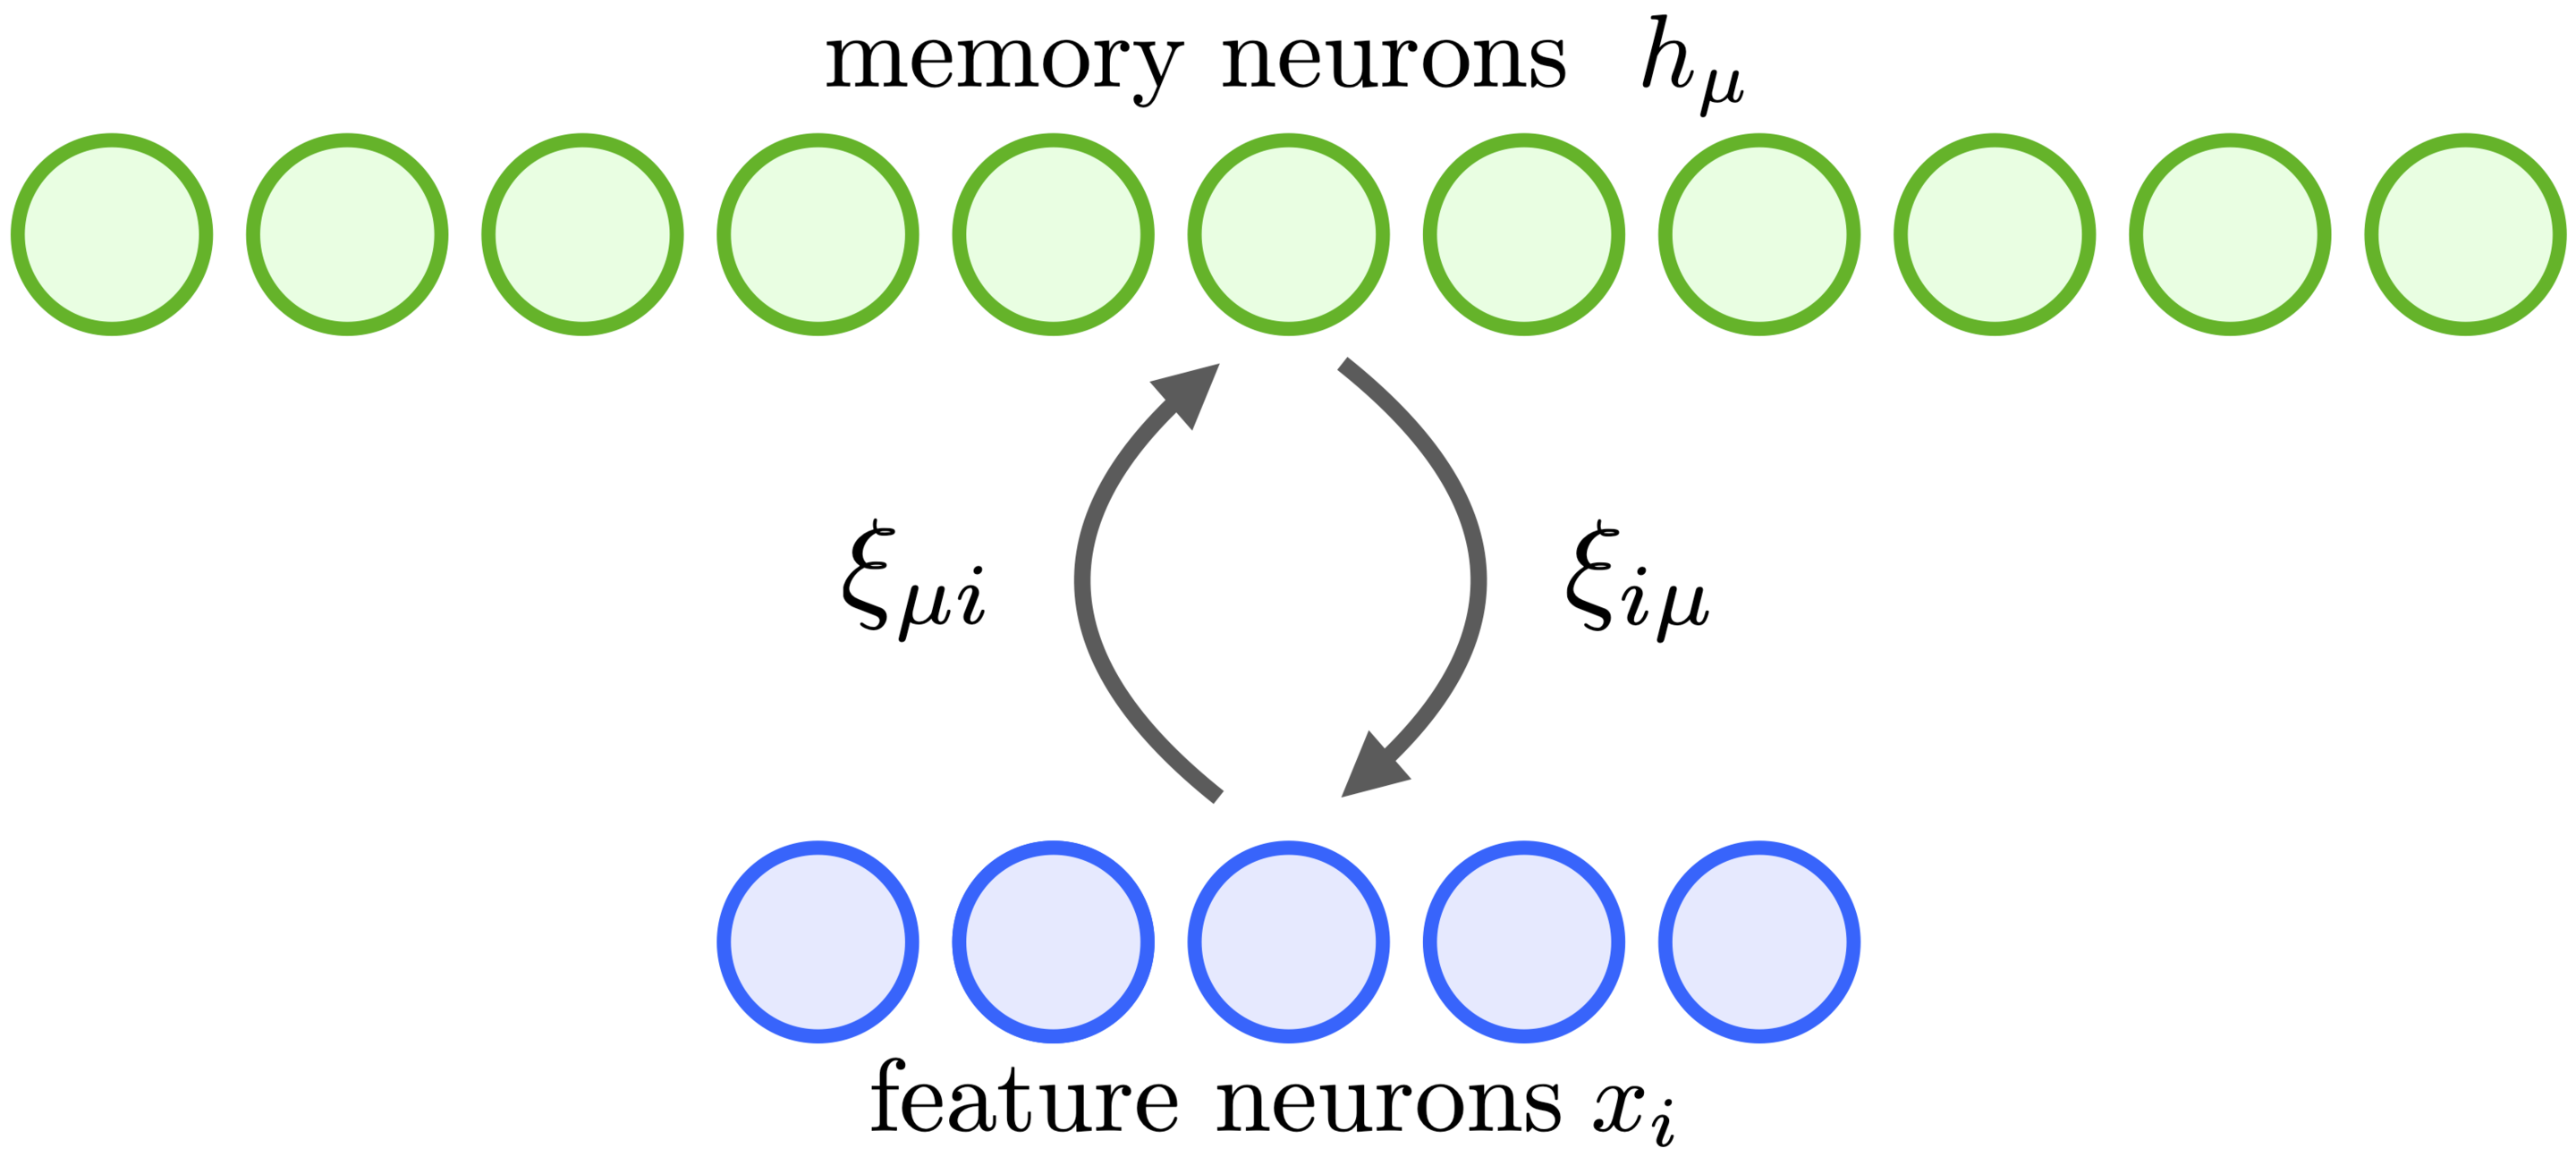
\includegraphics[width=0.7\linewidth]{pic/Modern_Hopfield_Network.png}
        \end{figure}
    \end{itemize}
\end{frame}

\begin{frame}
    \begin{itemize}[<+-| alert@+>] % 当然,除了alert,手动在里面插 \pause 也行
        \item Dans le domaine de \textit{l'apprentissage profond} : 
        \item Trois types de réseau neuronal :
        \begin{itemize}[<+-| alert@+>] % 当然,除了alert,手动在里面插 \pause 也行
            \item Réseau neuronal artificiel 
            \item Réseau neuronal de convolution
            \item Réseau neuronal récurrent
            \begin{figure}
                \centering
                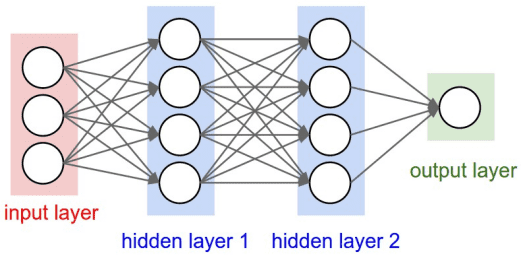
\includegraphics[width=0.5\linewidth]{pic/ffnet.png}
            \end{figure}
            \begin{figure}
                \centering
                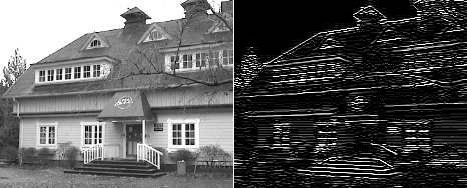
\includegraphics[width=0.5\linewidth]{pic/conv.jpeg}
            \end{figure}
        \end{itemize}
    \end{itemize}
\end{frame}

\section{Conclusion}

\begin{frame}[allowframebreaks]
    %\bibliography{ref}
    %\bibliographystyle{njupt}
    % 如果参考文献太多的话,可以像下面这样调整字体:
    % \tiny\bibliographystyle{alpha}
    \begin{itemize}
        \item Article \textit{d'Alan Turing} très fondateur en 1950.
        \item Construction de \textit{Perceptron} par \textit{Frank Rosenblatt} en 1958.
        \item Réseau inventé par \textit{John Hopfield} en 1982.
        \item Construction du MIND 1024 en 1985.
        \item Réseau de Hopfield :
            \begin{itemize}
                \item Ce en quoi cela consiste.
                \item Règle de mise à jour / calcul du nouvel état.
                \item Règle de Hebb, introduite par \textit{Donald Hebb} en 1949.
            \end{itemize}
        \item Réseaux Neuronaux d'aujourd'hui.
    \end{itemize}
\end{frame}

\begin{frame}
    \begin{center}
        {\Huge\calligra Merci !}
    \end{center}
\end{frame}

\end{document}